\documentclass{beamer}

\mode<presentation>
{

  \usetheme{Boadilla}
  \usecolortheme{whale}
  \setbeamercovered{transparent}
  
  \setbeamertemplate{footline}[frame number]{}
  \setbeamertemplate{navigation symbols}{}

}

\usepackage[english]{babel}
\usepackage[utf8]{inputenc}
\usepackage{times}
\usepackage[T1]{fontenc}

\usepackage{amsmath, amsthm, amssymb, amsfonts}
\usepackage{mathtools}

\usepackage{natbib}
\bibliographystyle{unsrtnat}

\usepackage{float}
\usepackage{bbm}
\usepackage{mathrsfs}

% ======== Alix notation =======
\def\th{\theta}
\def\eps{\epsilon}
\def\beq{\begin{equation}}
\def\eeq{\end{equation}}
\def\bdm{\begin{displaymath}}
\def\edm{\end{displaymath}}
\def\vsd{\vspace{0.1in}}
% ==============================

\usepackage{listings}




\title{Take Me Out to (Analyze) the Ballgame}
\subtitle{Visualization and Analysis Techniques for Big Spatial Data}
\author{Chris Comiskey} 
\institute{Oregon State University} 
\date{\today} 

% Delete this, if you do not want the table of contents to pop up at the beginning of each subsection:

\AtBeginSection[]
{
 \begin{frame}<beamer>{Outline}
   \tableofcontents[currentsection,currentsubsection]
 \end{frame}
}

% \AtBeginSubsection[]
% {
%  \begin{frame}<beamer>{Outline}
%    \tableofcontents[currentsection,currentsubsection]
%  \end{frame}
% }

\begin{document}

\begin{frame}
  \titlepage
\end{frame}

\section{Introduction}

\begin{frame}{Baseball, Baseball, Baseball} % ==================
\begin{columns}
\column{0.5\textwidth}
\begin{itemize}
\item Chris, rookie year
\end{itemize}

        \begin{figure}[H]
      	\centering
      	\includegraphics[scale=.65]{Images/CWC_Royals.pdf}
      	% Images only work with: setwd("~/Desktop/ResearchRepo/Seminar")
      	\end{figure}

\column{0.5\textwidth}
\begin{itemize}
\item Chris, Boston Red Sox
\end{itemize}
  \begin{figure}[H]
	\centering
	\includegraphics[scale=.3]{Images/RedSox.jpg}
	\end{figure}

\end{columns}
\end{frame}

\begin{frame}{Contributions Road map}{}
\begin{enumerate}
\addtolength{\itemsep}{0.5\baselineskip}
\item Variable-resolution heat maps, and {\bf varyres}
\item Interactive confidence intervals, and {\bf mapapp}
\item Approaches to Big N Spatial Generalized Linear Mixed Models (SGLMMs) for baseball data \\
  \begin{itemize}
  \addtolength{\itemsep}{0.5\baselineskip}
  \item Optimizing in Stan \citep{STANtheMan}
  \item Predictive Process Models (PPMs) \citep{Banerjee2008}
  \item Integrated Nested Laplace Approximations (INLA) \citep{Rue2009}
  \end{itemize}
\end{enumerate}

\end{frame}

\begin{frame}{Hitting Analytics, Then and Now} % ==================
\begin{columns}
\column{0.5\textwidth}
\begin{itemize}
\item $\text{``The Science of Hitting''}_{\text{1970}}$
\end{itemize}

        \begin{figure}[H]
      	\centering
      	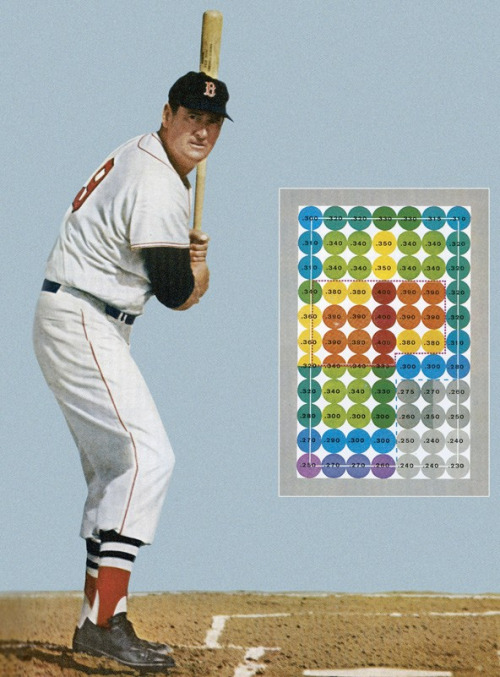
\includegraphics[scale=.22]{Images/Williams.jpg}
      	% Images only work with: setwd("~/Desktop/ResearchRepo/Seminar")
      	\end{figure}
      
\begin{itemize}
\item Iconic breakthrough, hitter
\item No data
\end{itemize}

\column{0.5\textwidth}
\begin{itemize}
\item The Statistics of Hitting
\end{itemize}
  \begin{figure}[H]
	\centering
	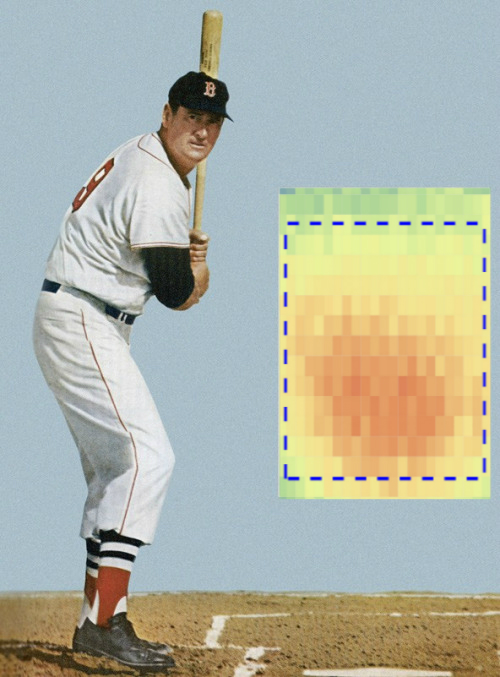
\includegraphics[scale=.22]{Images/WilliamsMother.jpg}
	\end{figure}
\begin{itemize}
\item PITCHf/x data, R, heat maps
\item SGLMMs, Stan, PPMs, INLA
\end{itemize}

\end{columns}
\end{frame}

\section{Varible-Resolution Heat Maps}

\begin{frame}{Empirical Success Probability Heat Map} % =============
\begin{columns}

\column{0.5\textwidth}

  \begin{figure}[H]
	\centering
	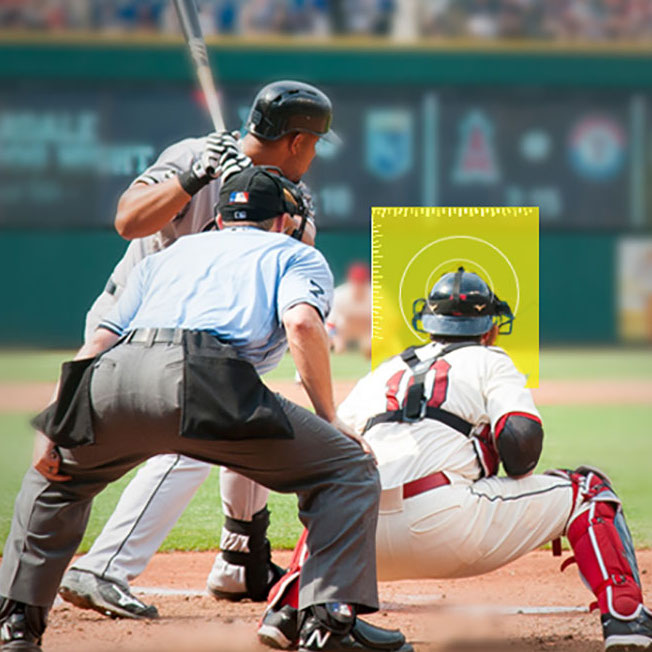
\includegraphics[scale=.26]{Images/StrikeZone3.jpg} 
	\end{figure}

\column{0.5\textwidth}
  \begin{figure}[H]
	\centering
	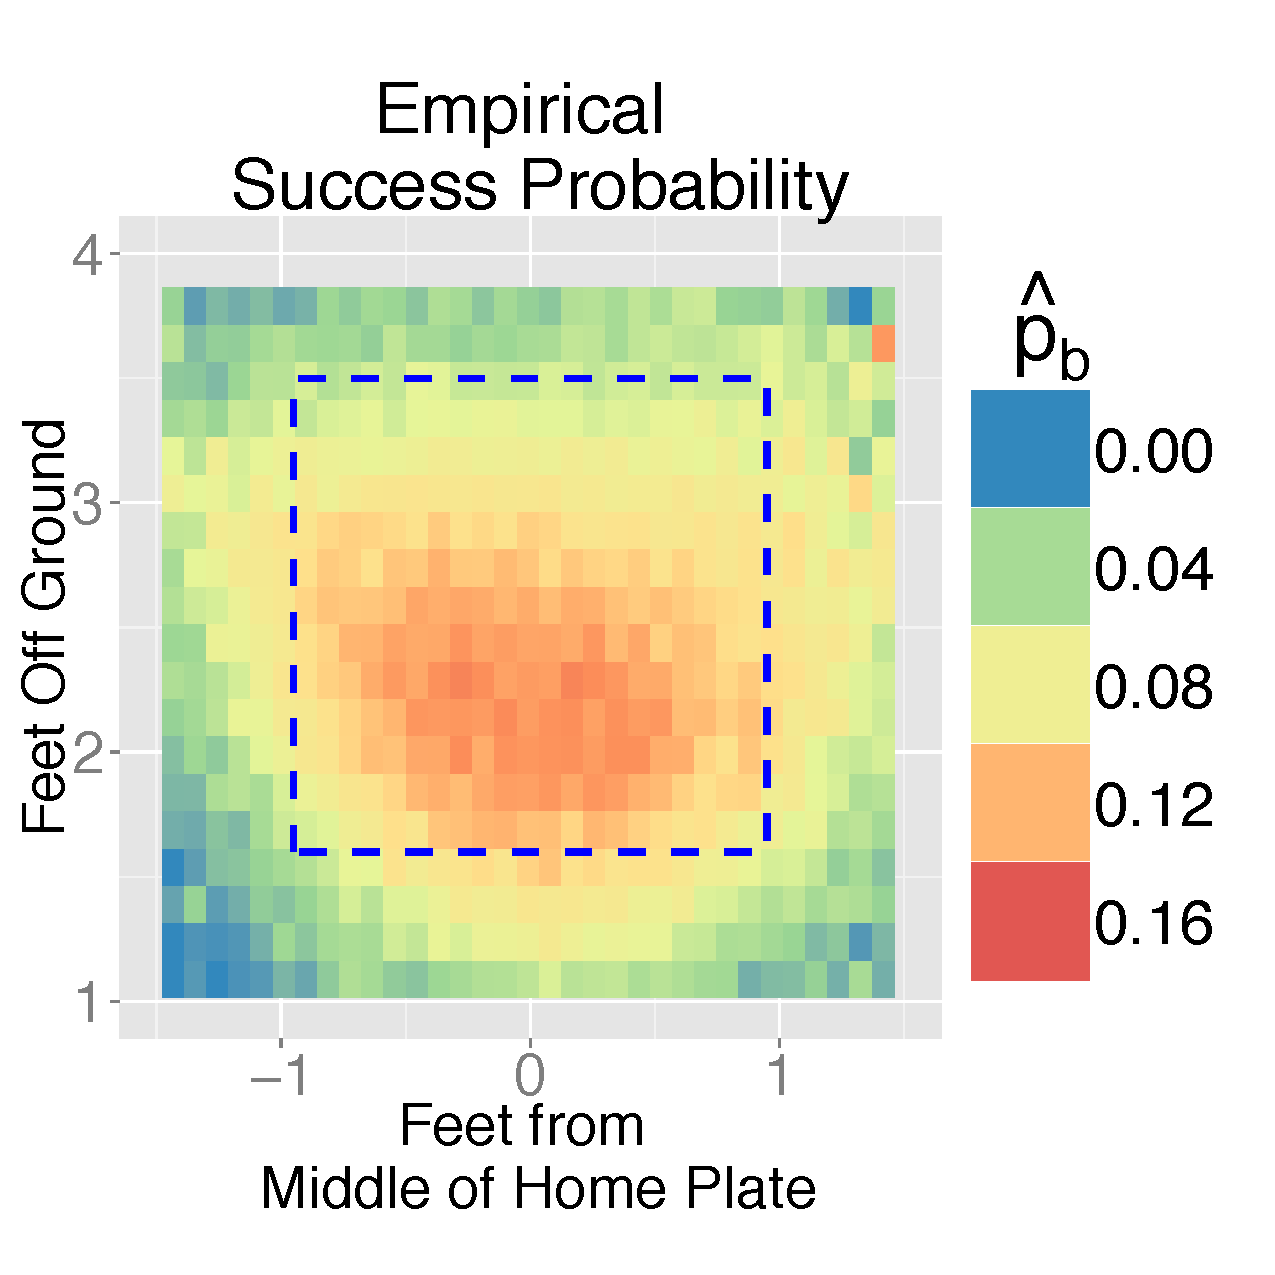
\includegraphics[scale=.07]{Images/Mothership.jpg} 
	\end{figure}
	
\end{columns}
\end{frame}

\begin{frame}{Empirical Success Probability Heat Map} % ====

\begin{itemize}
\addtolength{\itemsep}{0.5\baselineskip}
\item Swings: $i = 1,2,\ldots, N$; and $\pi_i = Pr(S_i = 1)$ where:
    \bdm
    S_i = \left\{\begin{array}{ll} 1; & \mbox{swing success} \\
    					 0; & \mbox{swing failure} \\ \end{array} \right.
    \edm

\item Pitch location $(x_i,y_i)$, grid boxes $G_1,G_2,\ldots,G_B$:
    \bdm
    N_b = \sum_{i=1}^N I_{(x_i,y_i) \in G_b}
    \edm
\item $\pi_b = \mbox{Pr(Swing success in }G_b)$, estimate with:
    \bdm
     p_b = \frac{1}{N_b} \sum_{i=1}^N S_i I_{(x_i,y_i) \in G_b}
    \edm
for $b = 1,2,\ldots,B$.
\end{itemize}
\end{frame}

\begin{frame}{Heat Map Resolution, Jhonny Peralta}{Compare Resolutions}
  \begin{figure}[H]
	\centering
	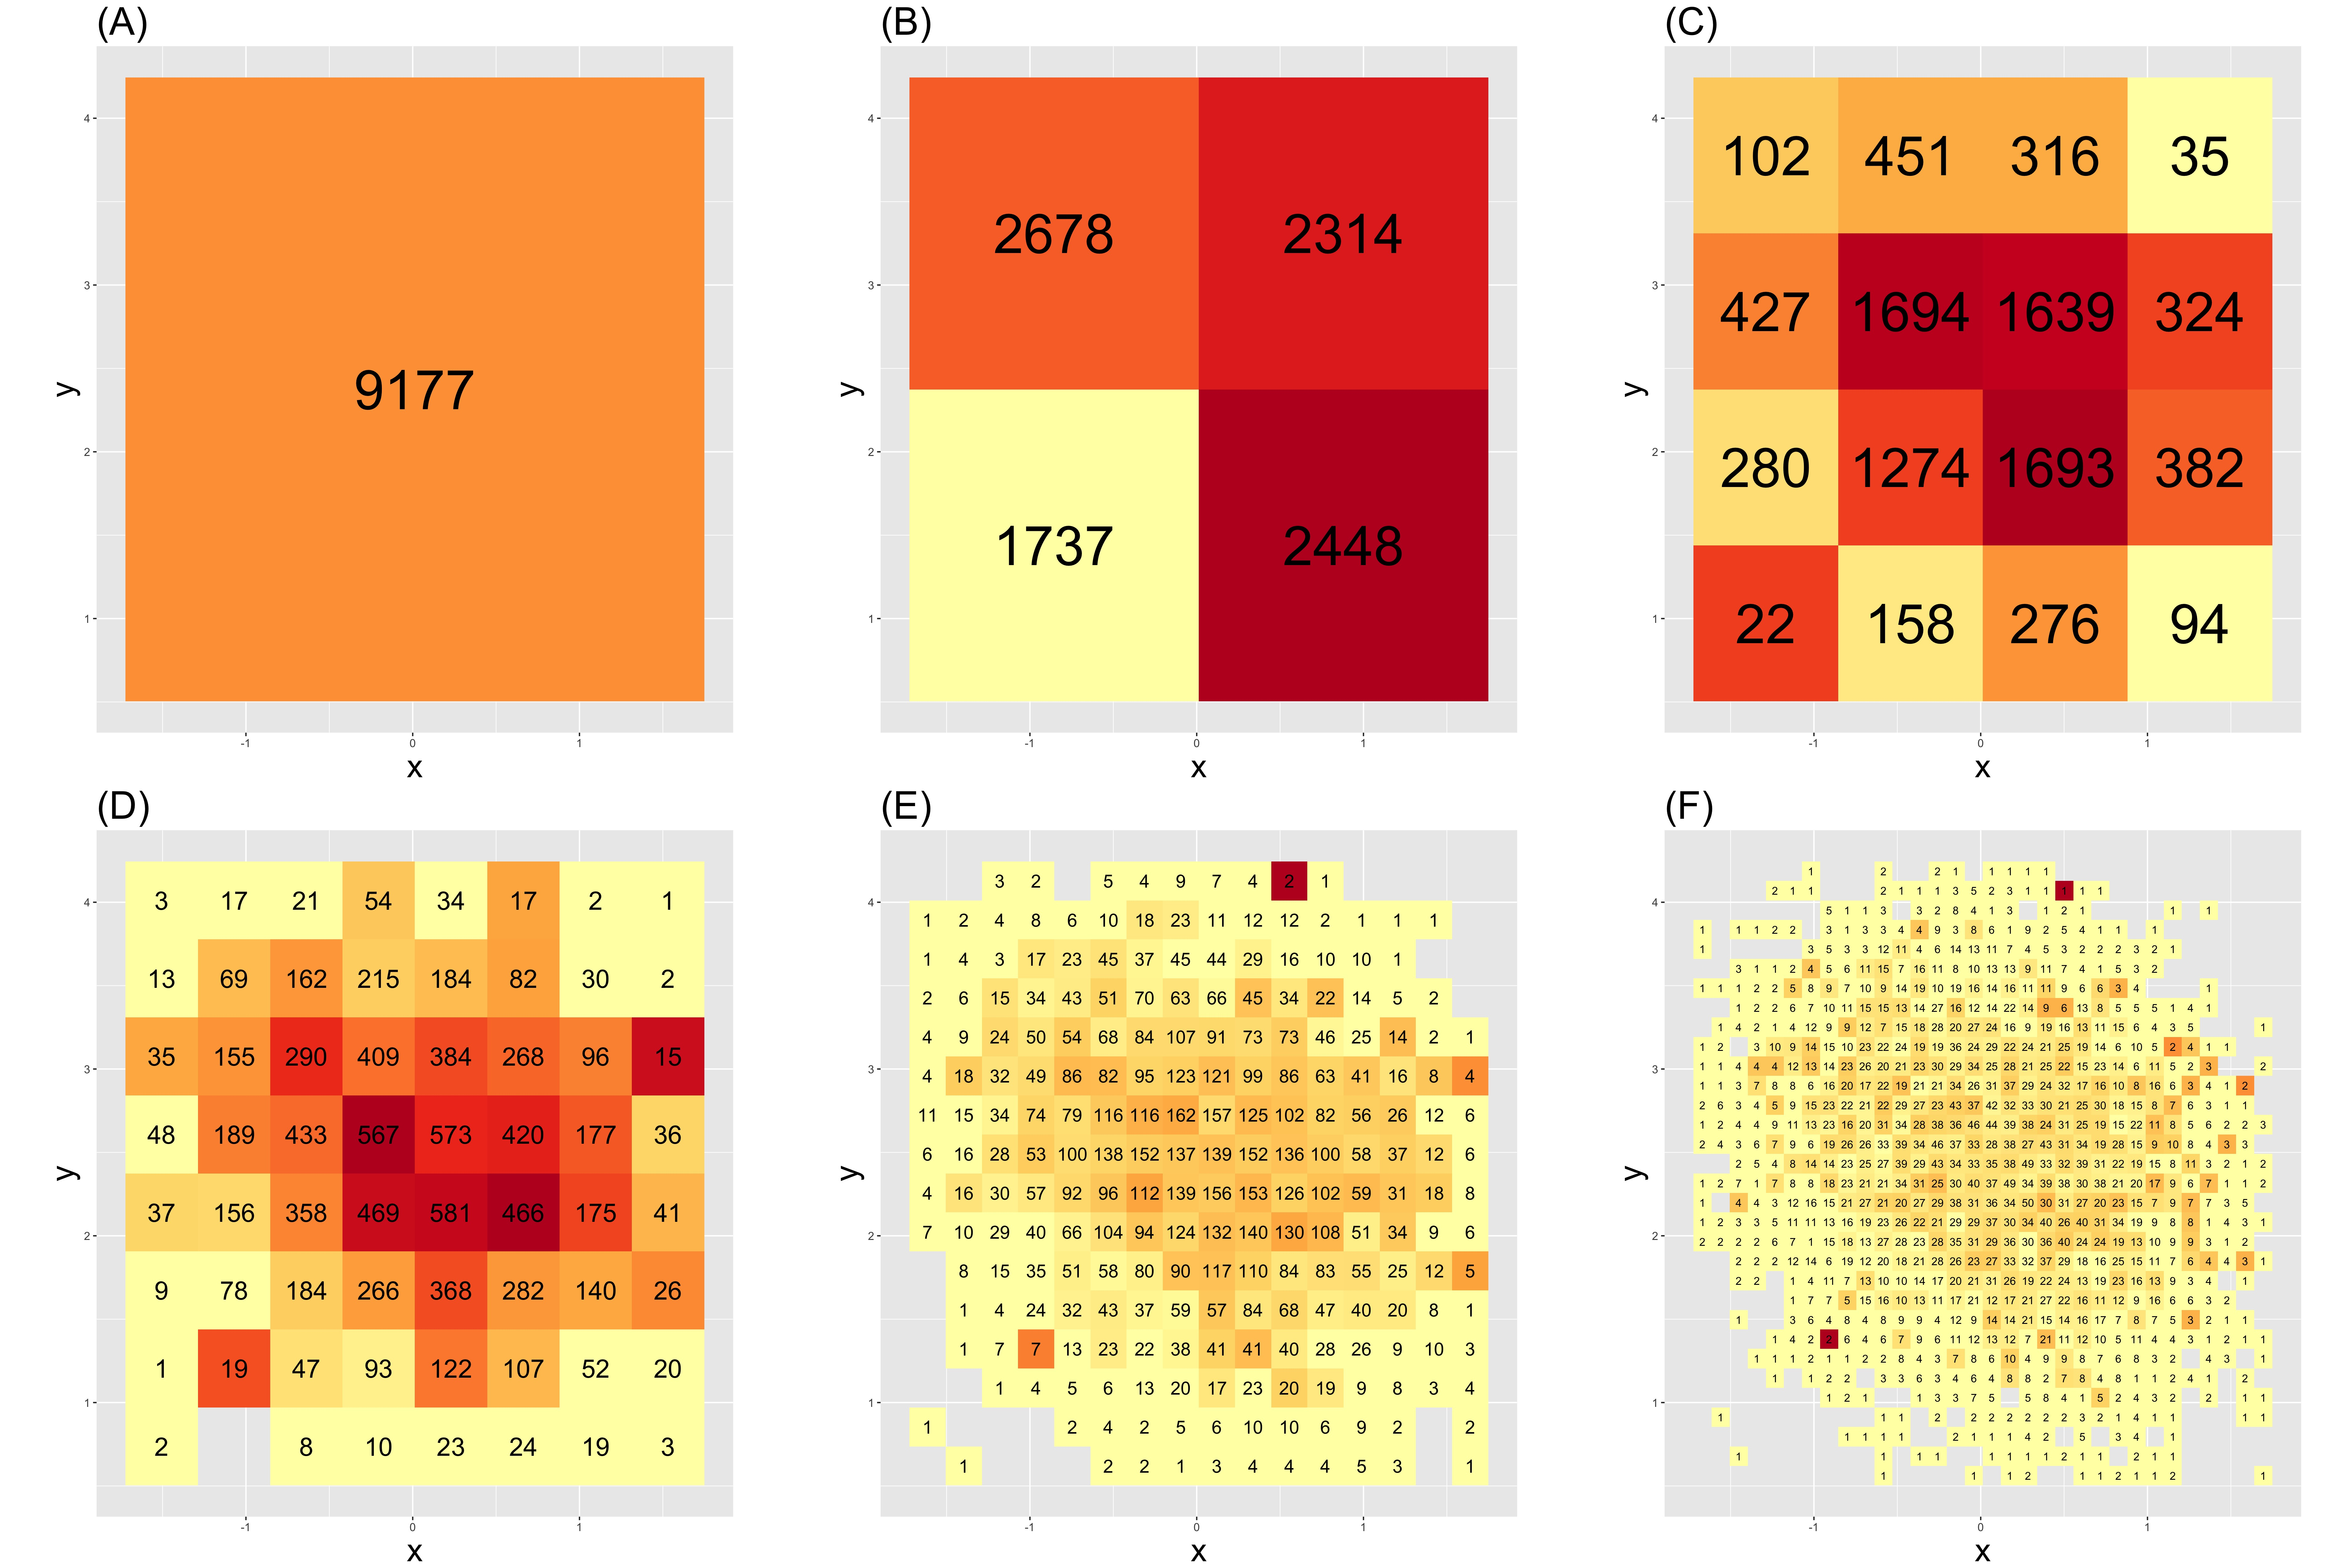
\includegraphics[scale=.0425]{Images/Chapter_VarRes.jpg}
	\end{figure}
\end{frame}

\begin{frame}{Heat Map Resolution, Jhonny Peralta}{Combine Resolutions}
  \begin{figure}[H]
	\centering
	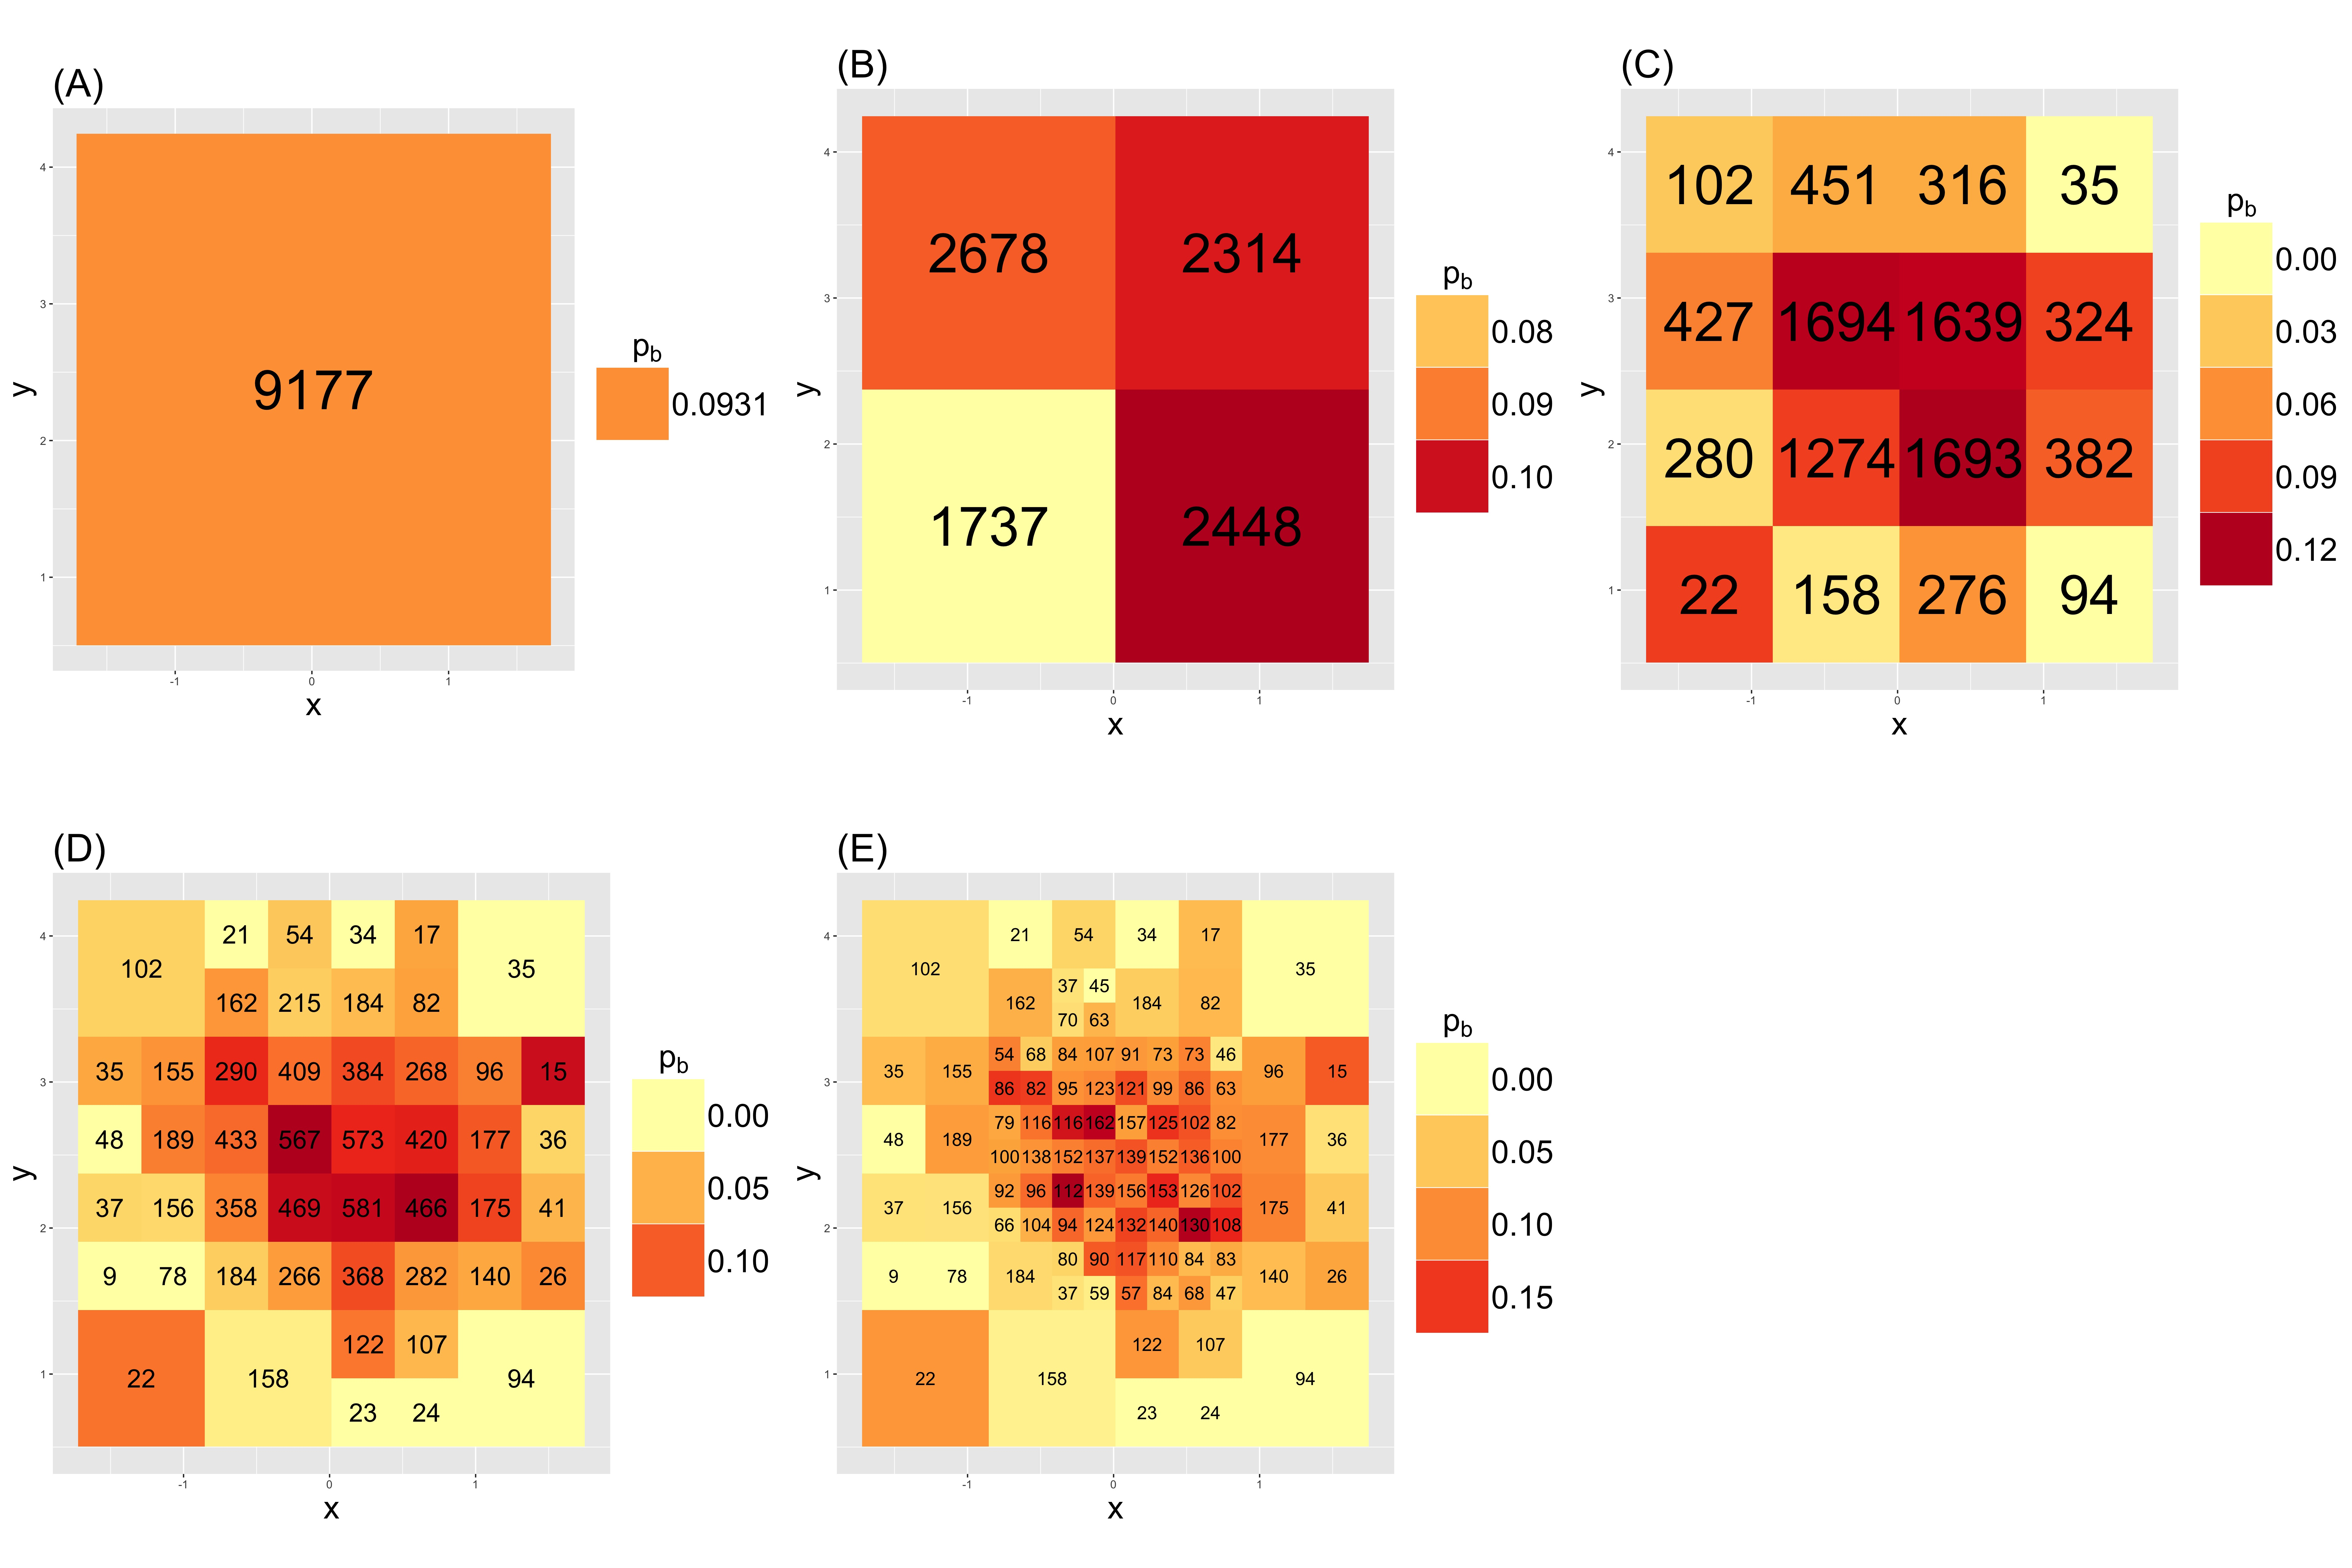
\includegraphics[scale=.0425]{Images/6_200.jpg}
	\end{figure}
\end{frame}

\begin{frame}{Best of Both (Spatial) Worlds}{}
\begin{itemize}
\addtolength{\itemsep}{0.5\baselineskip}
\item Location specific resolution, rather than one global resolution
\item Stopping rule $\iff$ {\bf sample size}* threshold
\item Local resolution conveys data density
  \begin{itemize}
  \addtolength{\itemsep}{0.5\baselineskip}
  \item Big box $\iff$ low density
  \item Bigger box, bigger variance*
  \end{itemize}
\item Choose subdivision algorithm
\end{itemize}
\end{frame}

\begin{frame}[fragile]{Variable-Resolution Algorithm}{Pseudo-code}
* Keep track of three containers: History, Current, Iteration
\begin{verbatim}
function(dataset, 
         fun = mean, # function to apply to box data
         cutoff,     # stopping rule threshold
         max ){      # maximum number of iterations
         
HISTORY_CONTAINER # store iterative results

CURRENT_CONTAINER: box centers, statistic, 
  box observations, box heights/widths, 
  box vert/horiz, upper/lower bounds

Add CURRENT_CONTAINER to HISTORY_CONTAINER
\end{verbatim}
\end{frame}

\begin{frame}[fragile]{Variable-Resolution Algorithm}{Pseudo-code}
\begin{verbatim}
WHILE(exists N_b > cutoff and ITERATION < max) {
  ITERATION CONTAINER <- list()
  
    FOR(All BOX_b in CURRENT CONTAINER){
      IF(BOX_b count > cutoff){ 
      
          Retrieve BOX_b data, subdivide/calculate 
            BOX_b sub-box info, add to 
            ITERATION CONTAINER  
      } 
    }  
    Update CURRENT_CONTAINER: remove obsolete boxes,
      add ITERATION CONTAINER boxes
    Add CURRENT CONTAINER to HISTORY CONTAINER 
  }

\end{verbatim}
\end{frame}

\begin{frame}{{\bf varyres}: An R Package}
Put something here
\end{frame}

\section{Interactive Heat Map Confidence Intervals}

\begin{frame}{Generalized Linear Model}{Logistic Link}
\begin{itemize}
  \addtolength{\itemsep}{0.5\baselineskip}
\item Pitch location: $\mathbf{s}_{i} = (x_{i},y_{i})$ 
\item Biomechanical covariate information: $\mathbf{X}_{i}(\mathbf{s}_{ij})$
\end{itemize}
$$Y_{ij}|\mathbf{X}_{i}(\mathbf{s}_{i}) \stackrel{ind}{\sim} \mbox{Bernoulli}(\pi_{i}) $$
$$
\log\left(\frac{\pi_{i}}{1-\pi_{i}}\right) = \mathbf{X}_{i}(\mathbf{s}_{i})\pmb{beta},
$$
\end{frame}

\begin{frame}{Logistic Regression Model}{Jhonny Peralta} % ======
$$Y_{ij}|\mathbf{X}_{i}(\mathbf{s}_{i}) \stackrel{ind}{\sim} \mbox{Bernoulli}(\pi_{i}) $$
$$ \log\left(\frac{\pi_{i}}{1-\pi_{i}}\right) = \mathbf{X}_{i}(\mathbf{s}_{i})\pmb{beta},
$$  
  \begin{figure}[H]
	\centering
	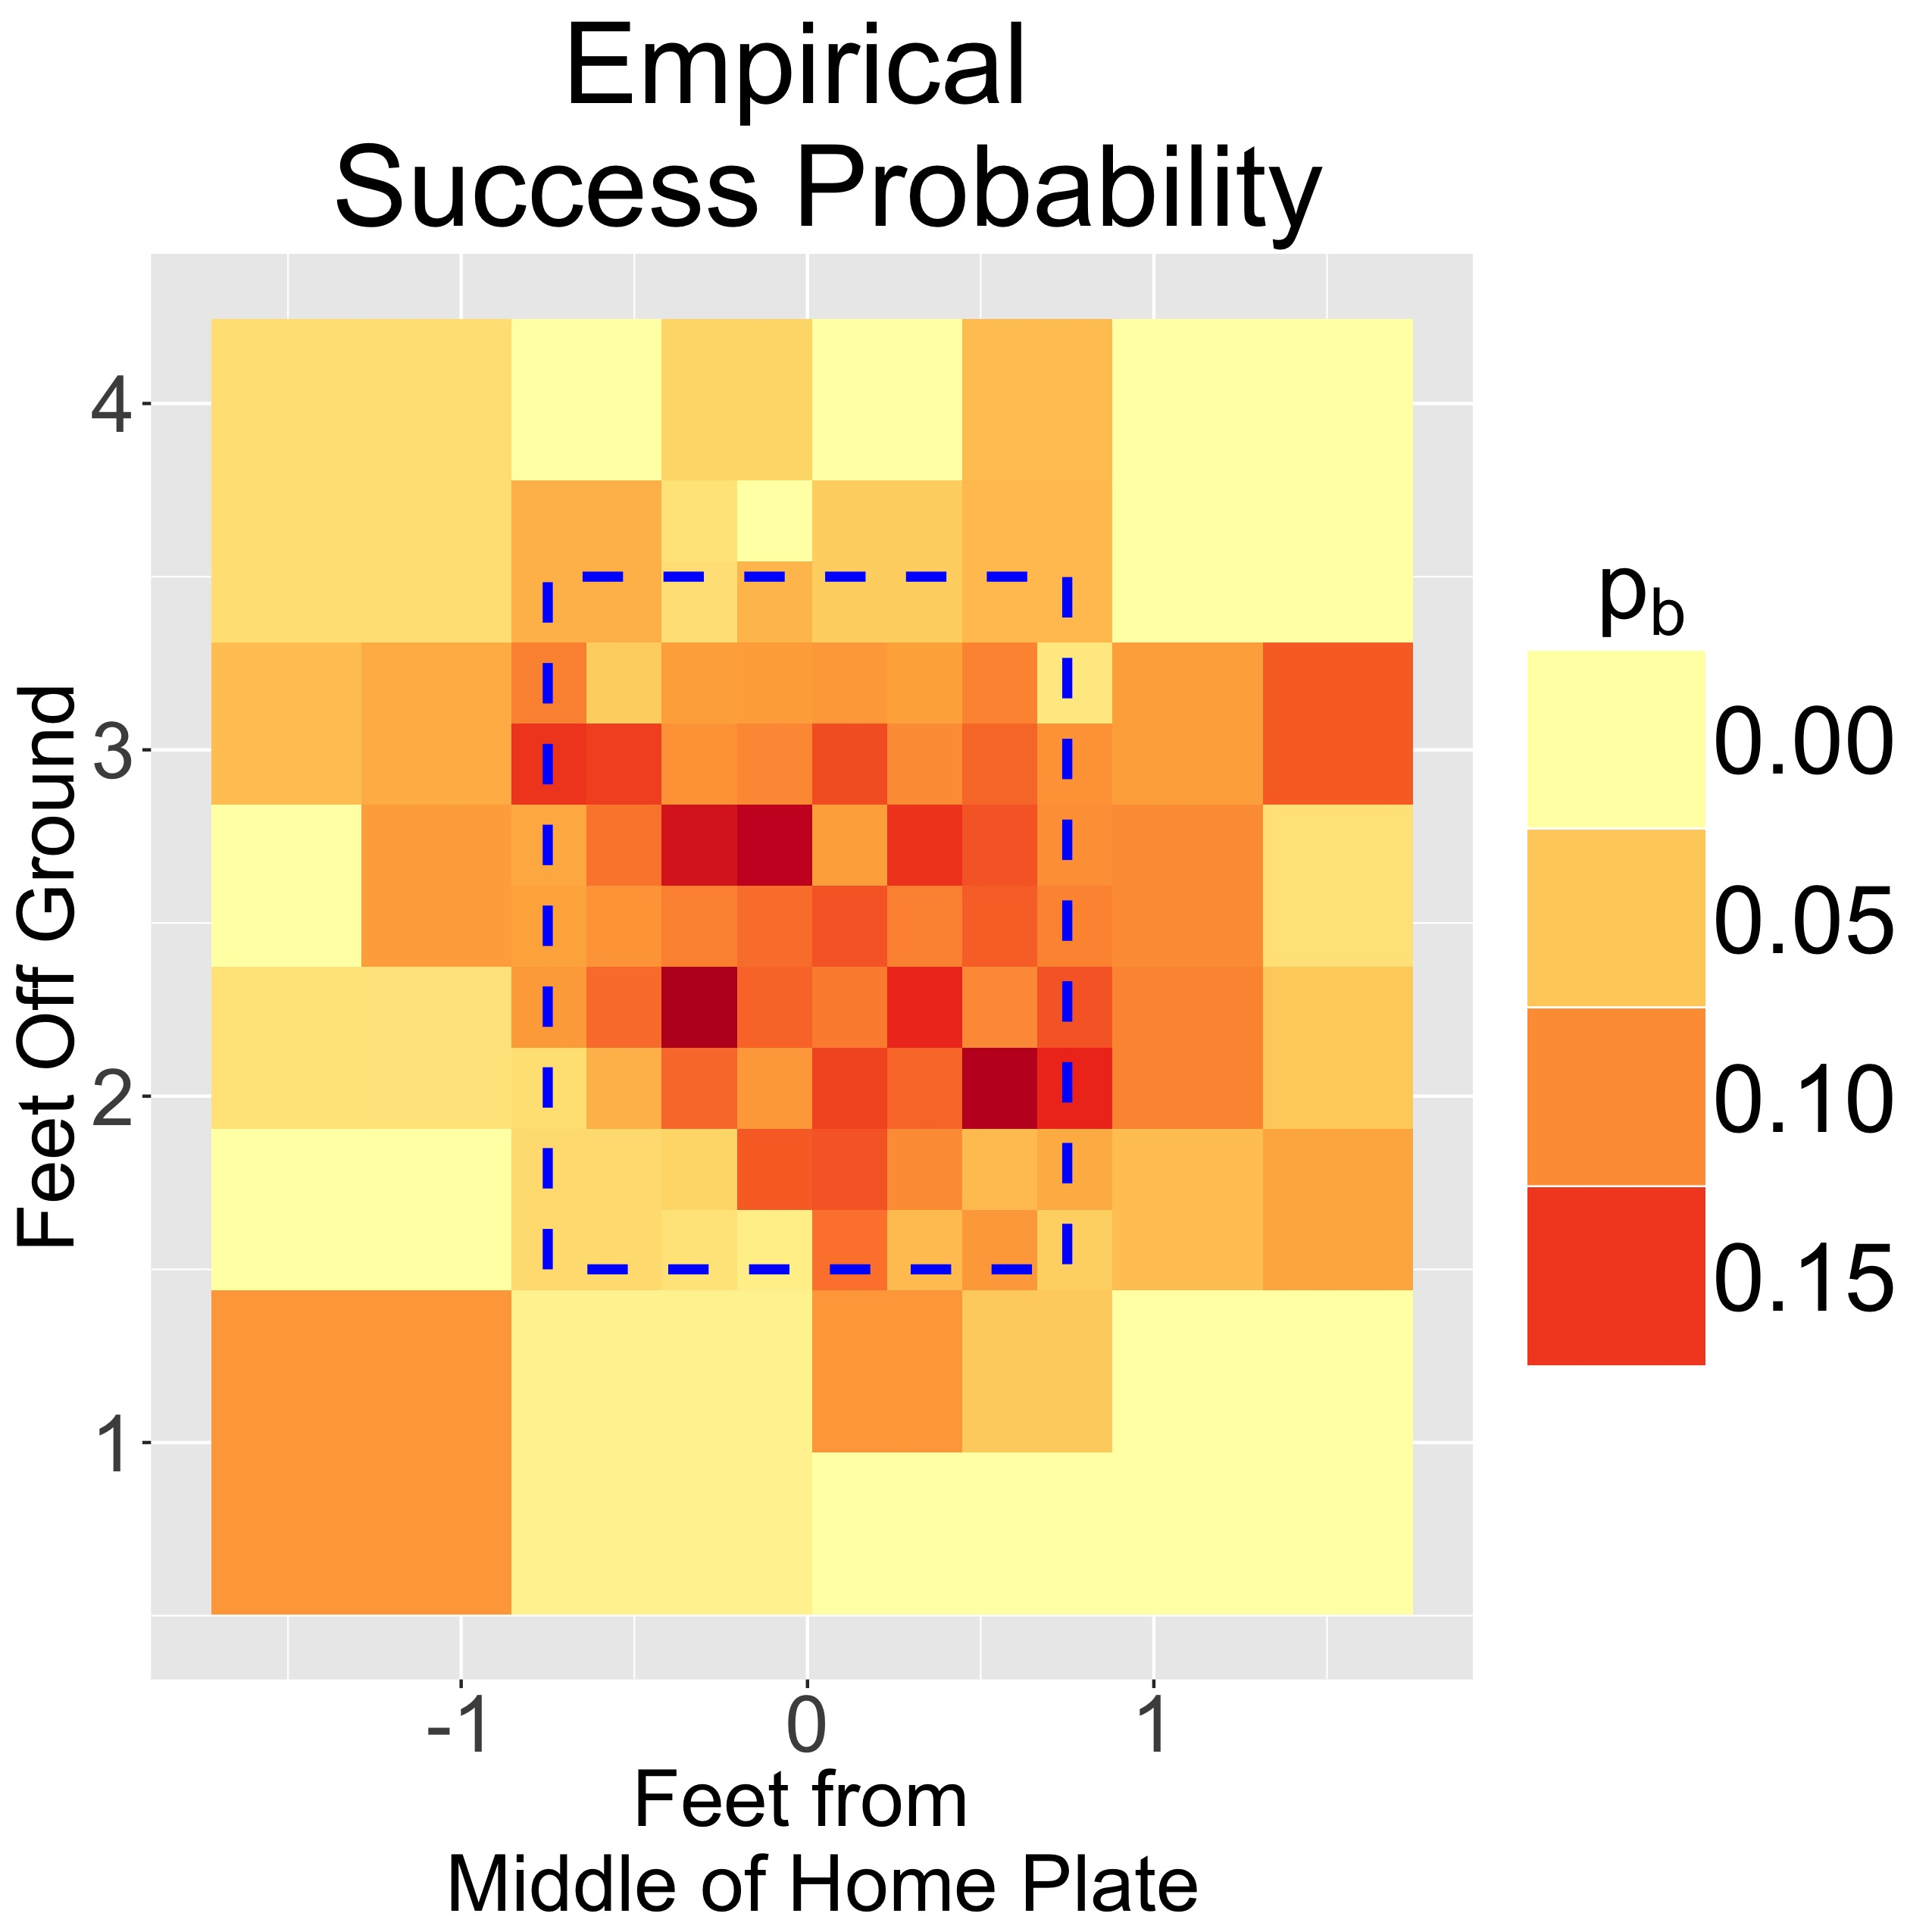
\includegraphics[scale=.06]{Images/Peralta_var-res2.jpg}
	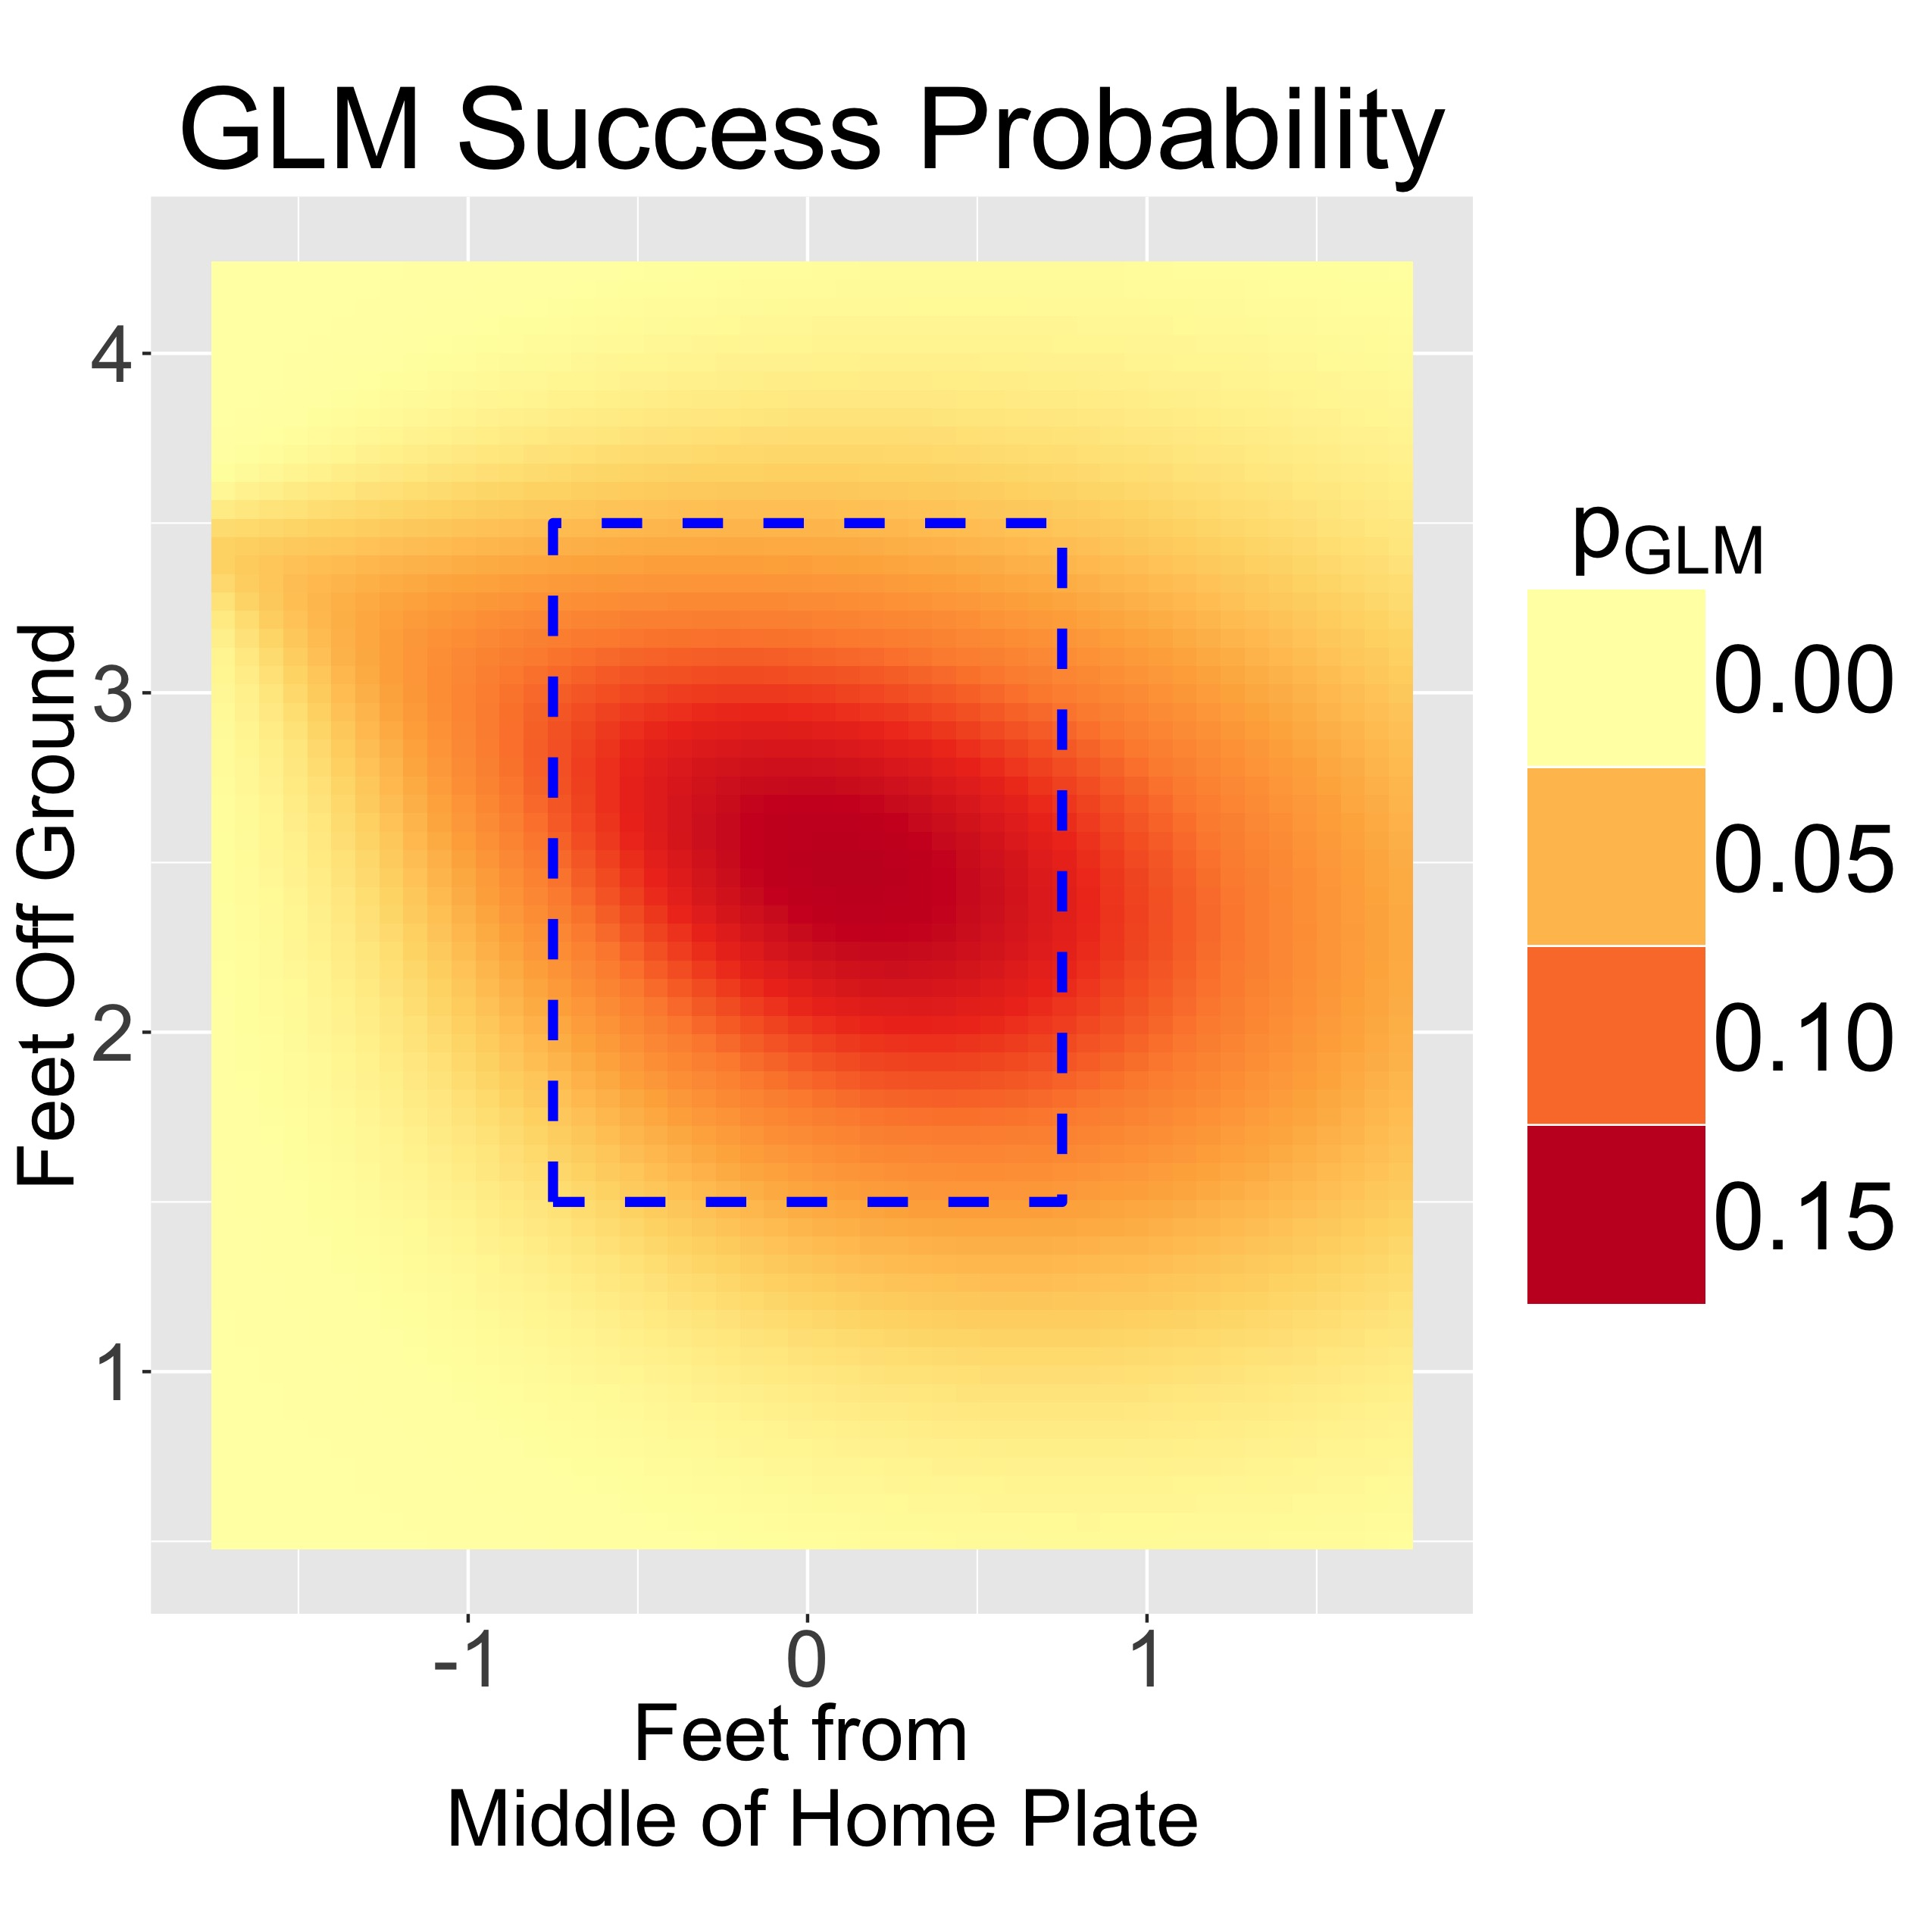
\includegraphics[scale=.06]{Images/Peralta_fit.jpg}
	\end{figure}

\end{frame}

\begin{frame}{Logistic Regression Model, Jhonny Peralta} % ======
  \begin{figure}[H]
	\centering
	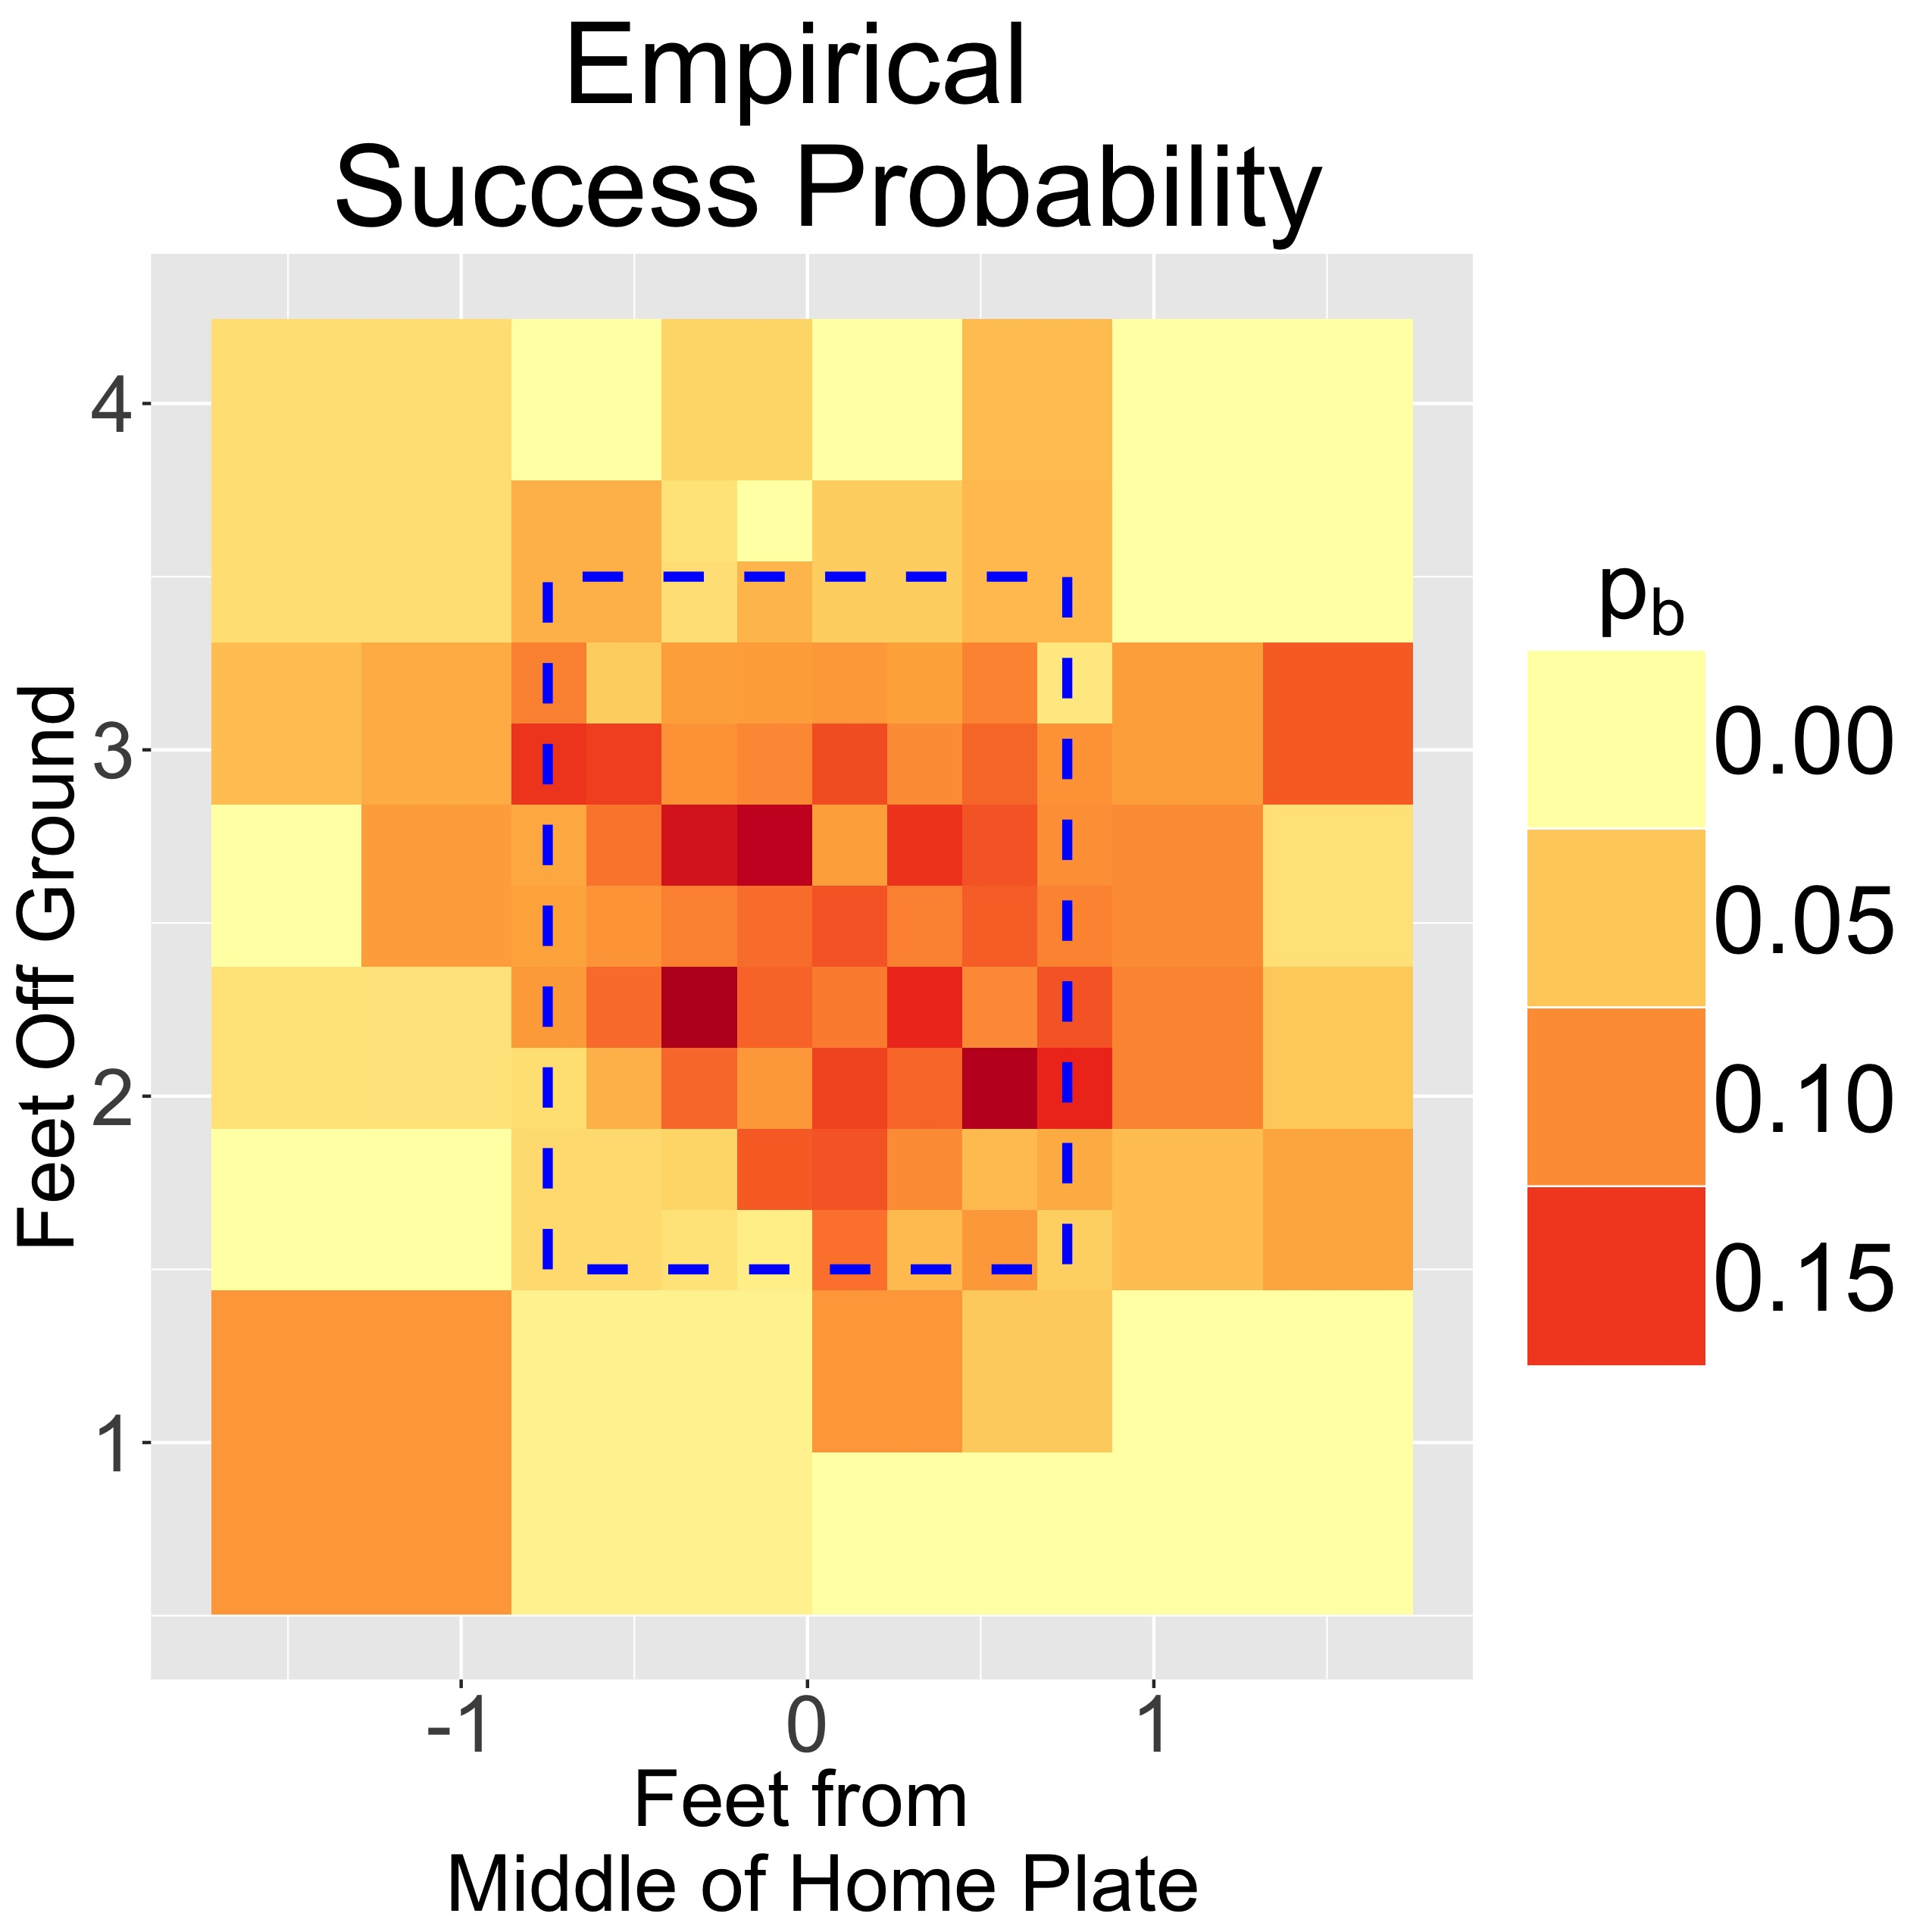
\includegraphics[scale=.05]{Images/Peralta_var-res2.jpg}
	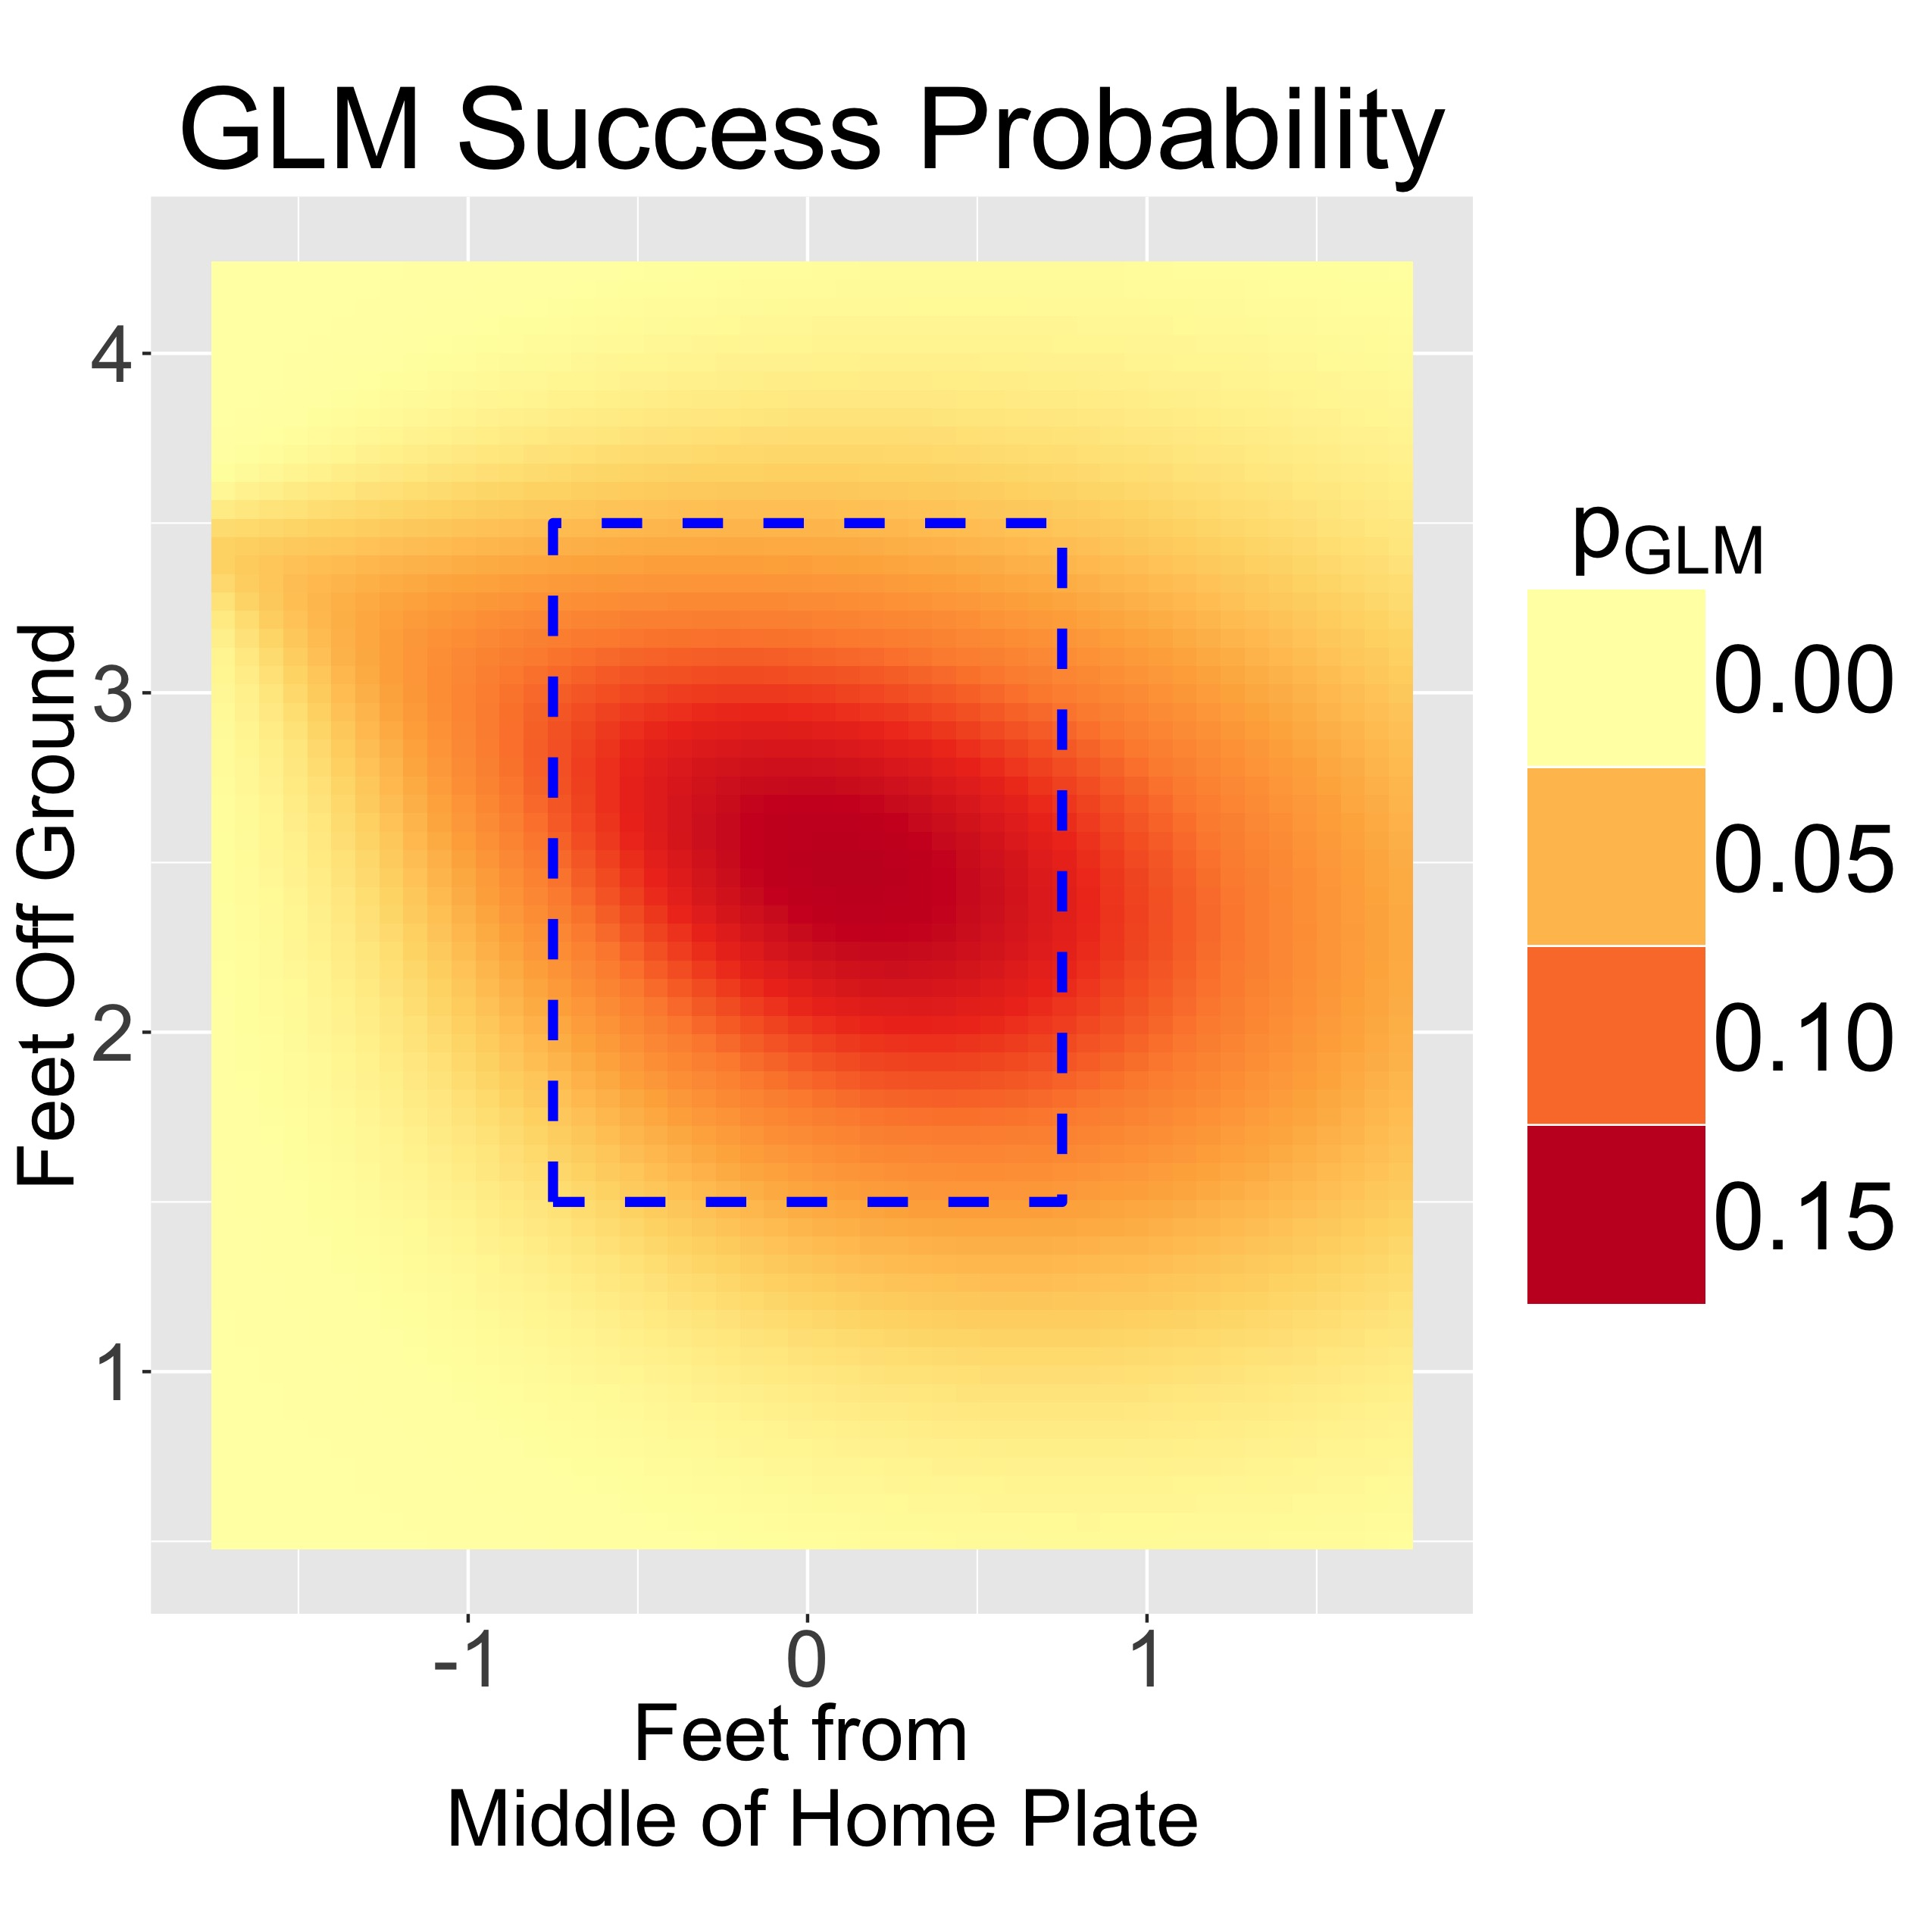
\includegraphics[scale=.05]{Images/Peralta_fit.jpg}
	\end{figure}
\begin{itemize}
\addtolength{\itemsep}{0.5\baselineskip}
\item Hosmer-Lemeshow (logistic regression) GOF test
  \begin{itemize}
  \addtolength{\itemsep}{0.5\baselineskip}
  \item Like Pearson $\chi^{2}$ test, but cont. covariates (no categories)
  \item $H_0$: Well fit \\ $H_A$: Lack of fit
  \item p-value = 0.8217
  \end{itemize}
\end{itemize}
\end{frame}

\begin{frame}{Interactive Confidence Intervals}{} % ======
  \begin{figure}[H]
	\centering
	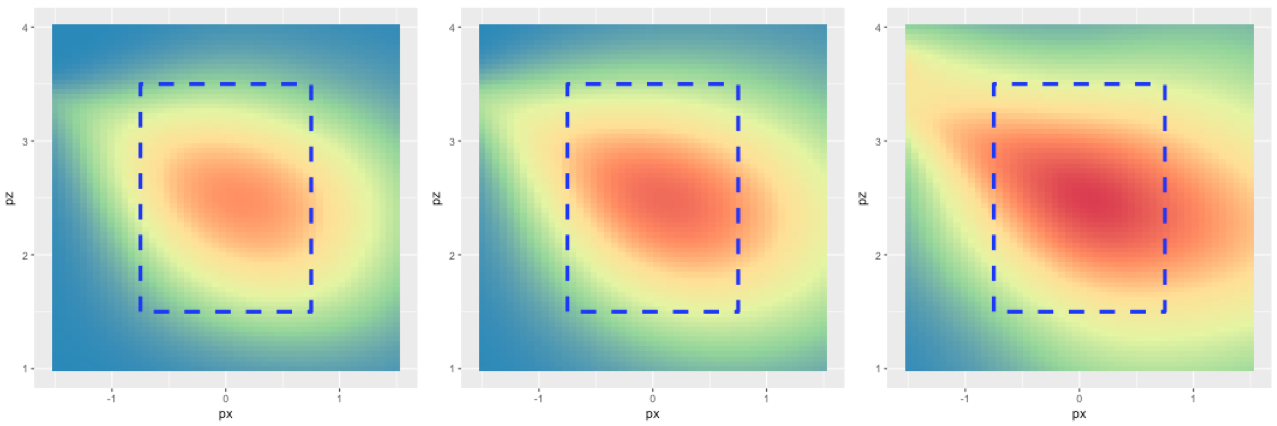
\includegraphics[scale=.275]{Images/99.png}
	\end{figure}
{\bf mapapp}: An R Package
\end{frame}

\section{Approaches to Big Data SGLMMs for Baseball Data}

\begin{frame}{GLM + Spatial Random Effect}{SGLMM}
For swings $i = 1, 2, \dots, N$:
$$ Y_{i}|\mathbf{X}_{i}(\mathbf{s}_{i}) \stackrel{ind}{\sim} \mbox{Bernoulli}(\pi_{i}) $$
$$\text{logit}(\pi_{i}|\pmb{s}_{i}) = \mathbf{X}_{i}(\mathbf{s}_{i})\beta + w(\pmb{s}_{i}) $$\begin{itemize}
\item $\pmb{w}(\pmb{s}) = (w(\pmb{s}_{1}), w(\pmb{s}_{2}), \dots, w(\pmb{s}_{N}))$  - vector of spatial random effects, where 
\item $w(\pmb{s}_{i})$ is the spatial random effect at location $\pmb{s}_{i}$. 
\end{itemize}
\end{frame}

\begin{frame}{Logistic Regression Model}{+ Spatial Random Effect} % ======

\bdm
Y_{i}|\mathbf{X}_{i}(\mathbf{s}_{i}) \stackrel{ind}{\sim} \mbox{Bernoulli}(\pi_{i})
\edm
\bdm
\log\left(\frac{\pi_{i}}{1-\pi_{i}}\right) = \mathbf{X}_{i}(\mathbf{s}_{i})\beta,
\edm
\begin{itemize}
\addtolength{\itemsep}{0.5\baselineskip}
\item Missing covariates
\item Tobler's First Law of Geography
\item Unexplained {\bf spatial} variation in the mean
\end{itemize}
\center{$\rightarrow$ Spatial Generalized Linear Mixed Model (SGLMM)}
\end{frame}

\begin{frame}{Spatial Generalized Linear Mixed Models}{} % ======
\begin{itemize}
\addtolength{\itemsep}{0.5\baselineskip}

\item SGLMM: $\text{logit}(\pi_{i}) = \pmb{X}_{i} \pmb{\beta} + w_{i}$
\item Gaussian Random Field (GRF)
  \begin{itemize}
  \item $\pmb{w} | \pmb{\theta} \sim MVN(\pmb{0}, \Sigma(\pmb{\theta}))$
  \end{itemize}

\item Covariance function
  \begin{itemize}
  \addtolength{\itemsep}{0.5\baselineskip}
  \item $ \Sigma(\phi, \sigma^{2})_{i,k} = \sigma^{2} exp(-||\pmb{s}_{i} - \pmb{s}_{k}||/\phi) $

  \item $||s_{i} - s_{k}||$ - Euclidean distance between $\pmb{s}_{i}$ and $\pmb{s}_{k}$
  \item $\sigma^{2}$ - scale parameter
  \item $\phi$ - range parameter.
  \end{itemize}
\end{itemize}
\end{frame}

\begin{frame}{Challenges} % ===============
$$ \text{logit}(p_{ij}) = \pmb{X}_{ij} \pmb{\beta} + w_{ij}$$
\begin{itemize}
\addtolength{\itemsep}{0.5\baselineskip}
\item We do not observe $p_{ij}$, instead Bernoulli$(p_{ij})$ trial outcome
\item We do not observe $n$ latent $w_{ij}$
\item $w_{ij}$ has a correlation structure, unknown correlation parameters $\rightarrow$ $p_{ij}$ has complicated correlation structure

\item Classical methods infeasible
  \begin{itemize}
  \item Imagine writing, maximizing the likelihood, partial derivatives
  \end{itemize}
\end{itemize}

  \begin{figure}[H]
	\centering
	\includegraphics[scale=.2]{Images/THOMAS_BAYES.jpg}
	\end{figure}

\end{frame}

% \begin{frame}{Bayesian Hierarchical Model}{} % ============
% 
% $$f(\theta|Y) \propto f(Y|\theta)f(\theta)$$
% 
% \begin{itemize}
% % \textcolor{blue}{f(\pmb{\alpha})} $
% \addtolength{\itemsep}{0.5\baselineskip}
% \item $Y_{ij}|p_{ij} \sim \text{Bernoulli}(p_{ij})$
% \item $\text{logit}(p_{ij}) = \pmb{X}_{ij} \pmb{\beta} + w_{ij}$
%   \begin{itemize}
%   \addtolength{\itemsep}{0.5\baselineskip}
%   \item $\pmb{\beta} \sim f_{\beta}(\pmb{\beta})$
%   \item $\pmb{w}_{ij}|(\sigma^{2}, \phi) \sim \text{MVN}(\pmb{0}, \Sigma_{\sigma^{2}, \phi})$
%   \item $\sigma \sim f_{\sigma}$, $\phi \sim f_{\phi}$
%   \end{itemize}        
% \item $f(\pmb{\beta}_{j}, \sigma, \phi|Y_{ij}) \propto  f(Y_{ij}|\pmb{\beta}_{j}, w) \cdot f_{\beta}(\pmb{\beta}_{j}) \cdot f(w|\sigma, \phi) \cdot f_{\sigma}(\sigma) \cdot f_{\phi}(\phi)$
% \end{itemize}
% 
% Great structure, now implementation.
% \end{frame}
% 
% \begin{frame}{Markov Chain Magic}
% Markov Chain Monte Carlo (MCMC) \\
% 
%         \begin{itemize}
%         \addtolength{\itemsep}{0.5\baselineskip}
%         \item Most popular Bayesian approach, by far 
%         \item Target and update parameters (or groups of) in sequence, procedurally reduced dimension
%         % Inference from posteriors of ``...arbitrarily large dimension, essentially by reducing the problem to one of recursively solving a series of lower-dimensional (often unidimensional) problems.''
%         \item Produce {\bf samples from posterior}; no closed form
%         % ``...work by producing not a closed form for posterior, but a sample of values $\{\theta^{(g)}, g = 1, \dots, G\}$ from this distribution.'' ($G$ = number of draws from posterior) 
%         \item It works!
%         \item Can take time, converges asymptotically, correlated draws
%         \end{itemize}
%         
% There's just one more thing.
% \end{frame}
% 
% \begin{frame}{One More Big (N) Problem}
% 
% \begin{itemize}
% \addtolength{\itemsep}{0.5\baselineskip}
% \item GRF $\pmb{w}_{j}$, recall $n \times n$ correlation matrix 
% \item Recall multivariate normal pdf
%     \begin{itemize}
%     \addtolength{\itemsep}{0.5\baselineskip}
%     \item $n \times n$ correlation matrix $\rightarrow$ invert $n \times n$ matrix
%     \item Jhony Peralta: 9172 $\times$ 9172!
%     \end{itemize}
% \item Iterative MCMC approach, invert lots of high dimension matrices
% \item Known as ``Big N'' problem
% \end{itemize}
% 
% How bad can it be? Plus, we have physics, and Stan!!
% \end{frame}
% 
% \begin{frame}{Hamiltonian Markov Chain (HMC) in Stan}
% \begin{itemize}
% \addtolength{\itemsep}{0.5\baselineskip}
% \item Proposal distribution - key component of MCMC algorithm
% \item Stan proposal machinery: HMC, from physics (molecular motion)
%   \begin{itemize}
%   \addtolength{\itemsep}{0.5\baselineskip}
%   \item $H(q(t),p(t)) = U(q(t)) + K(p(t))$
%   \item Total energy of a system
%   \item t = time
%   \item {\bf q = position (variables of interest)}, U = potential energy
%   \item p = momentum (auxiliary), K = kinetic energy
%   \end{itemize}
% \item $H(q,p) = -\text{log}f_{q}(q) + p^{T}\pmb{M}^{-1}p/2$
% \item Tidy partial derivatives
% \item {\bf Short version}: randomly sample momentum p (auxiliary), calculate new position q  --- that's your Metropolis proposal.
% \end{itemize}
% 
% Stan will be unstoppable!
% \end{frame}
% 
% \begin{frame}{Slow, Slow, Slow}{Meet Stan the snail.}
%   \begin{figure}[H]
% 	\centering
% 	\includegraphics[scale=1]{Images/Snail.jpg}
% 	\end{figure}
% 	
% 
% \end{frame}
% 
% \begin{frame}{Slow, Slow, Slow}{Meet Stan the snail.}
%   \begin{figure}[H]
% 	\centering
% 	\includegraphics[scale=1]{Images/Snail.jpg}
% 	\end{figure}
% 
% How slow? Prohibitively slow. Think geologic time scales; earth is 4.54 billion years old. 
% 
% \end{frame}
% 
% \begin{frame}{Optimization}{Give Stan a turbo-boost!}
%   \begin{figure}[H]
% 	\centering
% 	\includegraphics[scale=.2]{Images/FastSnail.jpg}
% 	\end{figure}
% \end{frame}
% 
% \begin{frame}{Stan Optimization}{}
% \begin{columns}
% \column{0.5\textwidth}  
%   \begin{figure}[H]
% 	% \centering
% 	\includegraphics[scale=.5]{Images/StanManCover.pdf}
% 	\end{figure}
% \begin{itemize}
% \item Stan Development Team Members
%       \begin{itemize}
%       \item Andrew Gelman
%       \item Bob Carpenter
%       \item Rob Trangucci
%       \end{itemize}
% \end{itemize}
% 
% 
% \column{0.5\textwidth}
%   \begin{figure}[H]
% 	\centering
% 	\includegraphics[scale=.4]{Images/Gelman.jpg}
% 	\end{figure}
% 	
% \end{columns}
% \end{frame}
% 
% \begin{frame}[fragile]{Stan Optimization}{}
% \begin{itemize}
% \addtolength{\itemsep}{0.5\baselineskip}
% \item Informative (sharp tailed) prior on exponential covariance length-scale parameter $\phi$ for model identifiability (normal or log-normal)
% \item Computing time/convergence - ``Complex models'' such as spatial hierarchical models require proper priors for all $\pmb{\beta}$ coefficients.
% \item QR factorization on covariate matrix X; reparameterize, adjust priors
% \begin{align*}
% \pmb{X} &= \pmb{QR} \\
% \pmb{X \beta} &= \pmb{QR \beta} \rightarrow \text{Let } \pmb{\theta} = \pmb{R \beta} \\
% \pmb{X \beta} &= \pmb{Q \theta} \\
% \pmb{\beta} &= \pmb{R^{-1}\theta}
% \end{align*}
% \end{itemize}
% \end{frame}
% 
% \begin{frame}[fragile]{Stan Optimization}{}
% \begin{itemize}
% \addtolength{\itemsep}{0.5\baselineskip}
% \item Add noise to the covariance matrix diagonal, ensure numerical positive-definiteness
% \item Cholesky decomposition and tactical reparameterization 
%     \begin{verbatim}
%     L = cholesky_decompose(Sigma);
%     Z ~ normal(0, 1);
%     Z_mod = L * Z;
%     Y ~ bernoulli_logit(Q*theta + Z_mod);
%     \end{verbatim}
% \item Matrix algebra and vectors, over ‘for loops’ and scalars
% \begin{verbatim}
% hit ~ bernoulli_logit(X*beta + Z)
% \end{verbatim}
% is faster than
% \begin{verbatim}
% for (n in 1:N)
%     hit[n] = bernoulli_logit(X[n]*beta[n] + Z[n]);
% \end{verbatim}
% \end{itemize}
% On your mark. Get set...
% \end{frame}
% 
% \begin{frame}{Go Stan 2.0!}
% 
%   \begin{figure}[H]
% 	\centering
% 	\includegraphics[scale=.5]{Images/Wheee.jpg}
% 	\end{figure}
% 
% \end{frame}
% 
% \begin{frame}{How Slow is Stan 2.0?}
% 
% \begin{itemize}
% \addtolength{\itemsep}{0.5\baselineskip}
% \item N = 1000: 7 hours 45 mins for 1500 draws
%   \begin{itemize}
%   \item Note: w/o spatial effect: 6 seconds.
%   \end{itemize}
% \item N = 2000 overnight, 350 draws
% \end{itemize}
%   \begin{figure}[H]
% 	\centering
% 	\includegraphics[scale=.32]{Images/Turtle.png}
% 	\end{figure}
% 
% \end{frame}
% 
% \begin{frame}{The ``Big N'' Problem Revisited}
% \begin{itemize}
% \addtolength{\itemsep}{0.5\baselineskip}
%   \item SGLMM computational costs
%   % \item $\mathcal{O}(n^{3})$ % ($t(n) \leq M \cdot n^{3}$ as $n \rightarrow \infty$)
%   \begin{itemize}
%   \addtolength{\itemsep}{0.5\baselineskip}
%   \item Increase at a rate of $\mathcal{O}(n^{3})$: 
%   $$t(n) \leq M \cdot n^{3} \text{ as } n \rightarrow \infty$$   
%   \item Spatial random effect covariance matrix $\Sigma$ is $n \times n$
%   \item Every iteration requires $\Sigma^{-1}$
%   \item Determinant of $\Sigma$
%   \end{itemize}
% \item Computational bottleneck
% \end{itemize}
% \end{frame}
% 
% \begin{frame}{Persistence}
% 
% \begin{columns}
% 
% \column{0.5\textwidth}
% 
% \begin{center}
% \Large Secret 7. You can do it. A PhD is 10\% intelligence and 90\%
% persistence.
% \end{center}
% 
% \column{0.5\textwidth}
%   \begin{figure}[H]
% 	\centering
% 	\includegraphics[scale=.5]{Images/Kearns.png}
% 	\end{figure}
% 
% \end{columns}
% \end{frame}
% 
% \begin{frame}{Predictive Process Models (PPMs)} {Dimension Reduction}
% NCAR workshop, Andrew Finley 
% 
%   \begin{itemize}
%   \addtolength{\itemsep}{0.5\baselineskip}
%   \item MSU Deptartments of Forresty and Geography
%   \end{itemize}
%   
% ``Gaussian predictive process models for large spatial data sets'' \citep{Banerjee2008}
% 
% \begin{itemize}
% \addtolength{\itemsep}{0.5\baselineskip}
% \item Competitive approach with computational advantages
% \item Project original process onto lower dimensioned subspace; generate parent process realizations at knots
% \item ``Spatial sampling design for parameter estimation of the covariance function'' \citep{Zhu2005}
% \end{itemize}
% \end{frame}
% 
% \begin{frame}{PPM Procedure}{Nuts and Bolts}
% \begin{align*}
% \text{logit}(p_{ij}|\pmb{s}_{ij}) &= \pmb{X}_{ij}(\pmb{s}_{ij}) \pmb{\beta}_{j} + w(\pmb{s}_{ij}) \\
% \pmb{w}(\pmb{s}) | \pmb{\theta} &\sim \text{GRF}(\pmb{0}, \pmb{C}(\pmb{\theta}))
% \end{align*}
% \begin{itemize}
% \addtolength{\itemsep}{0.5\baselineskip}
% \item $\pmb{w}(\pmb{s})$ - $n \times 1$ vector of random effects, at locations $\pmb{s}$ 
% \item $\pmb{0}$ - $n \times 1$ zero vector 
% \item $\pmb{C}(\pmb{\theta})$ - $n \times n$, symmetric, positive-definite covariance matrix
%     \begin{itemize}
%     \item $\pmb{\theta}$ - covariance parameters
%     \end{itemize}
% \item $C(\pmb{s}_{i}, \pmb{s}_{j}; \pmb{\theta})$ - covariance of random effects  at locations $\pmb{s}_{i}$ and $\pmb{s}_{j}$
%       \begin{itemize}
%       \addtolength{\itemsep}{0.5\baselineskip}
%       \item $C(\pmb{\theta}) = [C(\pmb{s}_{i}, \pmb{s}_{j}; \pmb{\theta})]_{i,j=1}^{n}$
%       \end{itemize}
% \end{itemize}
% \end{frame}
% 
% \begin{frame}{PPM Knots}
% \begin{itemize}
% \addtolength{\itemsep}{0.5\baselineskip}
% \item $\pmb{S}^{*} = \{\pmb{s}_{1}^{*}, \dots, \pmb{s}_{m}^{*}\}$ --- $m$ knot locations
%   \begin{itemize}
%   \item $m < < n$ 
%   \end{itemize}
% \item $\pmb{w}^{*} = \left[w(\pmb{s}_{i}^{*})\right]_{i=1}^{m}$ -- knot location random effects
% \item $\pmb{C}^{*}(\pmb{\theta}) = \left[C(\pmb{s}_{i}^{*}, \pmb{s}_{j}^{*})\right]_{i,j = 1}^{m}$ -- knot covariance matrix
%   \begin{itemize}
%   \item $m \times m$ --- much smaller dimension
%   \end{itemize}
% \item $\pmb{w}^{*}|\pmb{\theta} \sim \text{GRF}\{\pmb{0}, \pmb{C}^{*}(\pmb{\theta})\}$ -- $m$-dimensional GRF
% \end{itemize}
% 
% \end{frame}
% 
% \begin{frame}{PPM, Krig $w(\pmb{s}_{0})$}
% \begin{itemize}
% \addtolength{\itemsep}{0.5\baselineskip}
% \item Interpolate $w(\pmb{s}_{0})$ using: (i) $m$ knots, (ii) parent process covariance structure, (iii) kriging procedure
% \item  $\tilde{w}(\pmb{s}_{0})$ - interpolated random effect
% \begin{align*}
% \tilde{w}(\pmb{s}_{0}) &= E[w(\pmb{s}_{0})|\pmb{w}^{*}] \\
% &= \pmb{c}^{T}(\pmb{s}_{0};\pmb{\theta}) \cdot \pmb{C}^{*-1}(\pmb{\theta}) \cdot \pmb{w}^{*}
% \end{align*}
% \item $\pmb{c}(\pmb{s}_{0};\pmb{\theta}) = \left[C(\pmb{s}_{0}, \pmb{s}_{j}^{*}; \pmb{\theta})\right]_{j = 1}^{m}$ --- $m \times 1$ vector, $\text{Cov}(w(\pmb{s}_{0}), \text{ knots})$
% \item Spatially varying linear combination
% \item Minimize squared error loss function (linear predictors, GRFs) 
% \end{itemize}
% 
% Now replace $w(\pmb{s})$ with $\tilde{w}(\pmb{s})$.
% \end{frame}
% 
% \begin{frame}[fragile]{The Predictive Process! $\tilde{w}(\pmb{s})$}
% Another Gaussian Random Field
% \begin{align*}
% \tilde{\pmb{w}}(\pmb{s}) &\sim \text{GRF}\{0, \tilde{C}(\cdot)\} \\
% \tilde{C}(\pmb{s}, \pmb{s}'; \pmb{\theta}) &= \pmb{c}^{T}(\pmb{s};\pmb{\theta}) \cdot \textcolor{blue}{\pmb{C}^{*-1}(\pmb{\theta})} \cdot \pmb{c}(\pmb{s}';\pmb{\theta})
% \end{align*}
% And a predictive process model!
%     \begin{equation}
%     \text{logit}(p_{ij}|\pmb{s}_{ij}) = \pmb{X}_{ij}(\pmb{s}_{ij}) \pmb{\beta}_{j} + \tilde{w}(\pmb{s})
%     \end{equation}
%     \begin{itemize}
%     \item Note dimension of \textcolor{blue}{covariance matrix}.
%     \item Implement in \verb|spBayes| \citep{Finley2007}.
%     \item Faster?
%     \end{itemize}
% \end{frame}
% 
% \begin{frame}{PPMs, Plot and Results}
% 
% \begin{columns}
% \column{0.5\textwidth}
% 
%       \begin{itemize}
%       \addtolength{\itemsep}{0.5\baselineskip}
%       \item n = 500, knots = 97, 10K samples, $\approx$ 4 mins
%       \item n = 1000, knots = 97, 10K samples, $\approx$ 6.7 mins 
%       \item n = 1000, knots = 49, 30K samples, $\approx$ 7 mins 
%       \item n = 3000, knots = 49, 80K samples, $\approx$ 54 mins
% %      \item n = 9172, knots = 49, ``80,000 samples completed'' but the dreaded rainbow pinwheel never went away when computer tried to resuscitate in morning. We'll never know...
%       \end{itemize}
% 
% \column{0.5\textwidth}
%   \begin{figure}[H]
% 	\centering
% 	\includegraphics[scale=.29]{Images/Sample_PPM_fit.pdf}
% 	\end{figure}
% 
% \end{columns}
% \end{frame}
% 
% \begin{frame}{PPM, Plot and Results}
% 
% \begin{columns}
% \column{0.5\textwidth}
% 
%   \begin{figure}[H]
% 	\centering
% 	\includegraphics[scale=.29]{Images/Sample_GLM_fit.pdf}
% 	\end{figure}
% 	
% \column{0.5\textwidth}
%   \begin{figure}[H]
% 	\centering
% 	\includegraphics[scale=.29]{Images/Sample_PPM_fit.pdf}
% 	\end{figure}
% 
% \end{columns}
% \end{frame}
% 
% \begin{frame}{Current Work, SPDE-INLA}
% 
% \begin{itemize}
% \addtolength{\itemsep}{0.5\baselineskip}
% \item What about n = 9172?
% \item Approximation method, works well for Bayesian hierarchical models with latent GRF
% \item Essentially a two part process for continuous domain
%   \begin{itemize}
%   \item Part 1: SPDE
%   \item Part 2: INLA
%   \end{itemize}
% \item To n = 9172... and beyond!!
% \end{itemize}
%   \begin{figure}[H]
% 	\centering
% 	\includegraphics[scale=.02]{Images/BL.jpg}
% 	\end{figure}
% 
% \end{frame}
% 
% \begin{frame}{Approximation Part 1, SPDE}
% SPDE - Stochastic partial differential equation \citep{Lindgren2011}
% $$ (\kappa^{2} - \Delta)^{\alpha/2}x(\pmb{s}) = \mathcal{W}(\pmb{s})$$
% \begin{itemize}
% \addtolength{\itemsep}{0.5\baselineskip}
% \item Convert GRF to Gaussian {\bf Markov} Random Field (GMRF)
%     \begin{itemize}
%     \item Sparse precision matrix
%     \end{itemize}
% \item Finite Element Method: project SPDE onto basis representation    
% \item Triangular mesh, defines piecewise linear basis representation
% $$ \tilde{x}(\pmb{s}) = \sum_{k} \psi_{k}(\pmb{s})x_{k}$$
%                   \begin{itemize}
%                   \addtolength{\itemsep}{0.5\baselineskip}
%                   \item $\psi_{k}(\pmb{s})$ --- deterministic basis functions
%                   \item $x_{k}$ --- weights, explicit and sparse precision matrix
%                   \item $\tilde{x}(\pmb{s})$ approximates SPDE solution
%                   \end{itemize}
% \end{itemize}
% \end{frame}
% 
% % \begin{frame}{SPDE, A Picture Worth 1000 Equations}
% % 
% %   \begin{figure}[H]
% % 	\centering
% % 	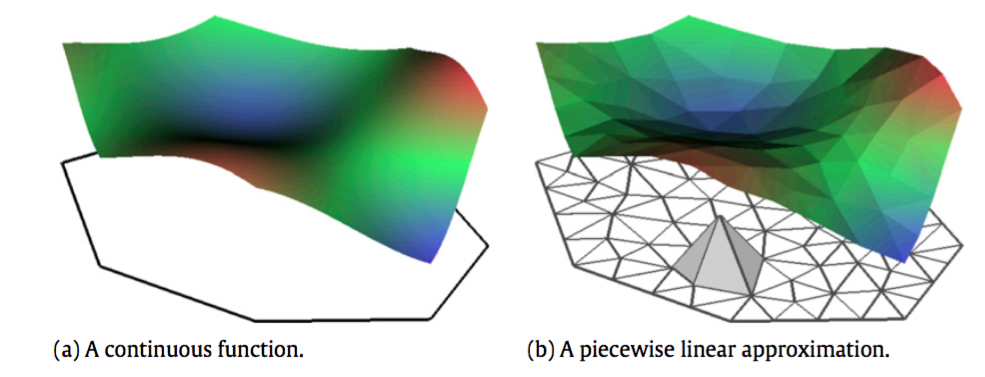
\includegraphics[scale=.3]{Images/PLBF.jpg}
% % 	\end{figure}
% % 	\citep{Simpson2012}
% % \end{frame}
% 
% \begin{frame}{Approximation Part 2, INLA}
% INLA - Integrated Nested Laplace Approximation \citep{Rue2009} \\ 
% 
%         \begin{enumerate}
%         \addtolength{\itemsep}{0.5\baselineskip}
%         \item Gaussian approximation: $\tilde{p}(\pmb{w}|\pmb{\theta, y})$
%         % (match mode and curvature at mode \citep{Rue2005})
%         % \item Posterior mode: $\pmb{w}^{*}(\pmb{\theta}) = \text{argmax}_{w}p(\pmb{w}|\pmb{\theta, y})$
%         \item Laplace approximation:
%         $$ p(\pmb{\theta} | \pmb{y}) \propto \frac{p(\pmb{\theta, y, w})}{p(\pmb{w}|\pmb{\theta, y})} \Big|_{\pmb{w} = \pmb{w}^{*}(\pmb{\theta})} \approx \frac{p(\pmb{\theta, y, w})}{\tilde{p}(\pmb{w}|\pmb{\theta, y})} \Big|_{\pmb{w} = \pmb{w}^{*}(\pmb{\theta})}$$
%         \begin{itemize}
%         \item $\pmb{w}^{*}(\pmb{\theta}) = \text{argmax}_{w}\tilde{p}(\pmb{w}|\pmb{\theta, y})$
%         \end{itemize}
% %        (unnormalized posterior at any point, numerically optimize for mode)
%         \item Numerical integration: 
%         $ p(\theta_{k} | \pmb{y}) \approx \int \tilde{p}(\pmb{\theta}|\pmb{y}) d\pmb{\theta}_{-k} $
%         \item Numerical integration: 
%         $ p(w_{j} | \pmb{y}) \approx \int \tilde{p}(w_{j}|\pmb{\theta, y})\tilde{p}(\pmb{\theta}|\pmb{y}) d\pmb{\theta} $
%         \end{enumerate}
% \end{frame}
% 
% \begin{frame}{Current Work, SPDE-INLA}
% \begin{itemize}
% \addtolength{\itemsep}{0.5\baselineskip}
% \item Implement in R-INLA \citep{Lindgren2015}
% \item Computational costs - increase at a rate of $\mathcal{O}(n^{3/2})$
% \item Trade-offs - speed for bias (Binomial data)
% \end{itemize}
% \end{frame}
% 
% \begin{frame}{Next Steps}
% \begin{itemize}
% \addtolength{\itemsep}{0.5\baselineskip}
% \item Cool SPDE-INLA pictures
% \item Model evaluation, scoring rules \citep{Bickel2007}
% \item Cross validation study
% \item Variable-resolution heat map R package?
% \item Dynamic Heat Map CIs -- R package?
% \end{itemize}
% \end{frame}
% 
% \begin{frame}{}
% \begin{center}
% \Huge{Thanks for listening. \\
% Questions?}
% \end{center}
%   \begin{figure}[H]
% 	\centering
% 	\includegraphics[scale=.105]{Images/Alix.jpg}
% 	\includegraphics[scale=.055]{Images/Ewan.jpg}
% 	\end{figure}
% \end{frame}

\bibliography{Baseball}



\end{document}







